%----------------------------------------------------------------------------------------

\part{Capítulo dos}
\graphicspath{ {2_Capitulo/img/ejemplos/},{2_Capitulo/img/explicacion/}, {W_Varios/2_Portada_capitulos} }

%----------------------------------------------------------------------------------------
%	CHAPTER 2
%----------------------------------------------------------------------------------------

\chapterimage{2_Capitulo/img/portada/ima2} % Chapter heading image
\chapter{Interés Compuesto}

%------------------------------------------
%Tabla de Fórmulas
%------------------------------------------

\section{Mapa Mental}
\begin{center}
   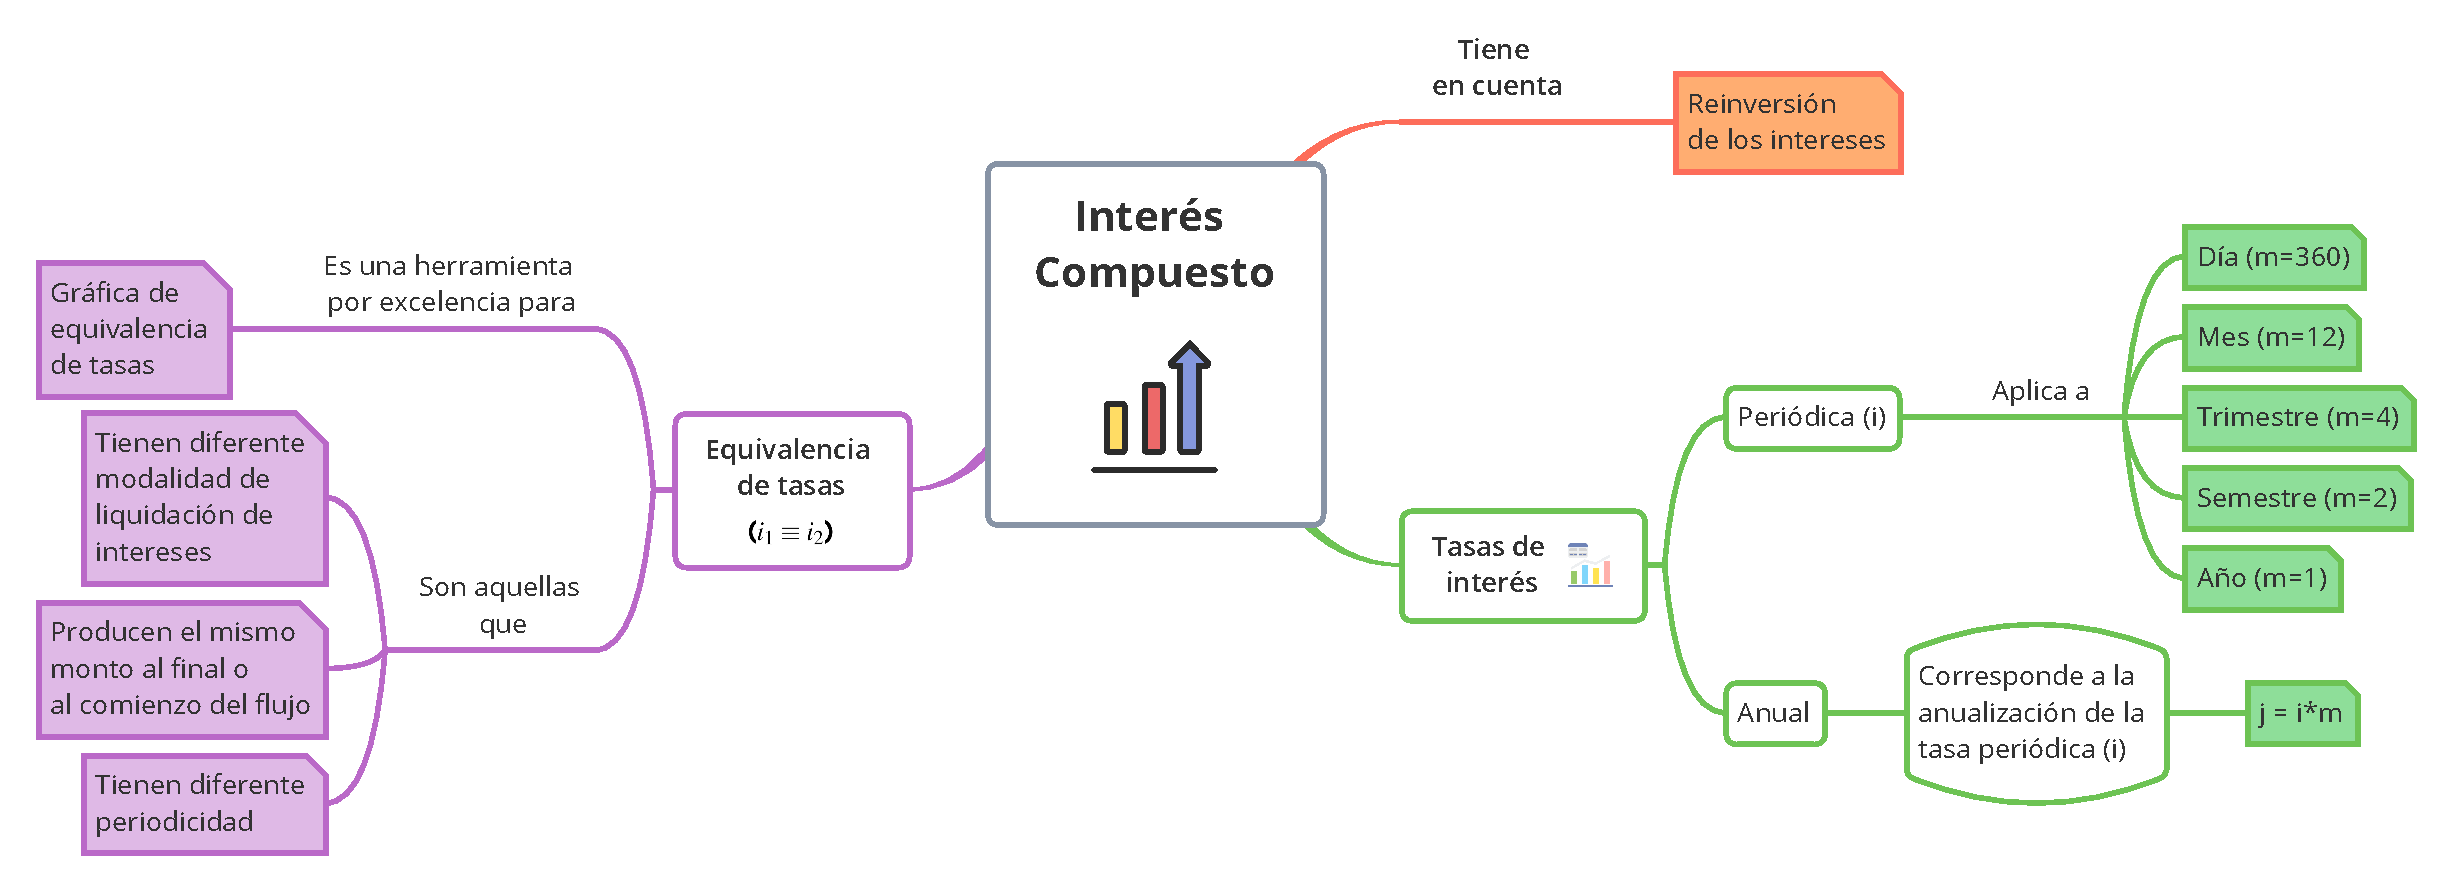
\includegraphics[height = 5.6 cm]{Mapa Mental 2.1.pdf}\\
\end{center}
\clearpage
\section{{Fórmulas del Capítulo}}
\begin{spacing}{1.3}
   \begin{center}
      \begin{tabular}{ |p{4cm}|p{5cm}| p{5cm}|}
         \hline
         \rowcolor{orange!50}
         \begin{center}\textbf{Fórmula} \end{center}   & \begin{center} \textbf{Nombre}\end{center} & \begin{center} \textbf{Excel} \end{center} \\ \hline
         F = $P(1+i)^n$                                & Valor futuro                               & VF(i;n;;VA,0)                              \\ \hline
         P = $\frac{F}{(1 + i)^{n}}$                   & Valor presente                             & VA(i;n;;VF,0)                              \\ \hline
         j = i(m)                                      & Tasa periódica anualizada                  & TASA.NOMINAL(i;m)                          \\ \hline
         ${(1 + i_{1})^{m_1}}$ = ${(1 + i_{2})^{m_2}}$ & Equivalencia de tasas                      & TASA(m;;-1;1+i)                            \\ \hline
      \end{tabular}
   \end{center}
\end{spacing}
\section{Interés compuesto}
Es la acumulación de intereses producidos por un capital inicial a una tasa de interés durante períodos determinados.\\

% ejemplo1
%%%%%%%%%%%%%%%%%%% EJERCICIO 1a %%%%%%

%\newpage %USAR SOLO SI EL SOLUCIÓN QUEDA SOLO Y ES NECESARIO BAJARLO A LA SIGUIENTE PAGINA
\textbf{Solución.}\\
%La tabla ira centrada
\begin{center}
	\renewcommand{\arraystretch}{1.6}% Margenes de las celdas
	%Creación de la cuadricula de 3 columnas
	\begin{longtable}[H]{|c|c|c|}
		%Creamos una linea horizontal
		\hline
		%Definimos el color de la primera fila
		\rowcolor[HTML]{FFB183}
		%%%%% INICIO ASIGNACIÓN PERIODO FOCAL %%%%%%%
		%%%%%%%%%% INICIO TITULO
		%Lo que se hace aquí es mezclar las 3 columnas en una sola
		\multicolumn{3}{|c|}{\cellcolor[HTML]{FFB183}\textbf{1. Asignación período focal}}  \\ \hline
		\multicolumn{3}{|c|}{$pf = \textit{0 ptv}$}   \\\hline
		%%%%%%%%%% FIN TITULO
		%%%%% INICIO DECLARACIÓN DE VARIABLES %%%%%%%
		%%%%%%%%%% INICIO TITULO
		%Lo que se hace aquí es mezclar las 3 columnas en una sola
		\multicolumn{3}{|c|}{\cellcolor[HTML]{FFB183}\textbf{2. Declaración de variables}}   \\ \hline
		%%%%%%%%%% FIN TITULO
		%%%%%%%%%% INICIO DE MATEMÁTICAS
		%Cada & hace referencia al paso de la siguiente columna
		\multicolumn{2}{|c|}{$ \hspace{2 cm} VP= 200.000 \ COP \hspace{2 cm}$}       & $ i  \equiv  8\% \textit{ ptv}$ \\
		\multicolumn{2}{|c|}{$ \hspace{2 cm} j \equiv 32\% \ \textit{natv} \hspace{2 cm}$} & $n=\textit{4 ptv}$ \\
		\multicolumn{2}{|c|}{$ \hspace{2 cm} R = ? COP  \hspace{2 cm}$}              &  \\ \hline
	
		
		%%%%%%%%%% FIN DE MATEMÁTICAS
		%%%%% FIN DECLARACIÓN DE VARIABLES
		
		
		%%%%% INICIO FLUJO DE CAJA
		\rowcolor[HTML]{FFB183}
		\multicolumn{3}{|c|}{\cellcolor[HTML]{FFB183}\textbf{3. Diagrama de flujo de caja}} \\ \hline
		%Mezclamos 3 columnas y pondremos el dibujo
		%%%%%%%%%%%%% INSERCIÓN DE LA IMAGEN
		%Deberán descargar las imágenes respectivas del drive y pegarlas en la carpeta
		%n_capitulo/img/ejemplos/1/capitulo1ejemplo1.pdf  (el /1/ es el numero del ejemplo)
		\multicolumn{3}{|c|}{ 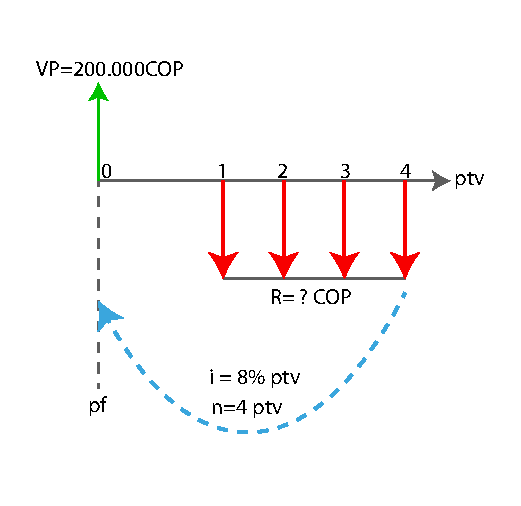
\includegraphics[trim=-78 -5 -78 -5]{7_Capitulo/img/ejemplos/1/Capitulo7-Ejercicio1.pdf} }
		
		
		\\ \hline
		%%%%%%%%%%%%% FIN INSERCIÓN DE IMAGEN
		%%%%%FIN FLUJO DE CAJA
		
		
		
		%%%%% INICIO DECLARACIÓN FORMULAS
		%%%%%%%%%%% INICIO TITULO
		\rowcolor[HTML]{FFB183}
		\multicolumn{3}{|c|}{\cellcolor[HTML]{FFB183}\textbf{4. Declaración de fórmulas}}    \\ \hline
		%%%%%%%%%%% FIN TITULO
		%%%%%%%%%%% INICIO MATEMÁTICAS
		
		\multicolumn{3}{|c|}{$VP=R(\frac{1-(1+i)^{-n}}{i}) \hspace{0.4 cm} \textit{Valor presente de una serie uniforme vencida}$} \\ \hline
		
		%%%%%%%%%% FIN MATEMÁTICAS
		%%%%%% INICIO DESARROLLO MATEMÁTICO
		\rowcolor[HTML]{FFB183}
		%%%%%%%%%%INICIO TITULO
		\multicolumn{3}{|c|}{\cellcolor[HTML]{FFB183}\textbf{5. Desarrollo matemático}}       \\ \hline
		%%%%%%%%%% FIN TITULO
		%%%%%%%%%% INICIO MATEMÁTICAS
		\multicolumn{3}{|c|}{$ 200.000 \ COP=R(\frac {1-(1+0.08)^{-4}} {8\% ptv}) $ \hspace{0.2 cm} $\rightarrow$ \hspace{0.2 cm} $ R= 60.384,16 \ COP $} \\ \hline
		
		%%%%%%%%%% FIN MATEMÁTICAS
		%%%%%% FIN DESARROLLO MATEMÁTICO
		%%%%%% INICIO RESPUESTA
		\rowcolor[HTML]{FFB183}
		%%%%%%%%%%INICIO TITULO
		\multicolumn{3}{|c|}{\cellcolor[HTML]{FFB183}\textbf{6. Respuesta}}   \\ \hline
		%%%%%%%%%% FIN TITULO
		%%%%%%%%%% INICIO RESPUESTA MATEMÁTICA
		\multicolumn{3}{|c|}{$\mathbf{R= 60.384,16 \ COP}$}
		\begin{comment}
		\multicolumn{3}{|p{\textwidth}|}{
		$F_{4} = F_{5} = 21.609,84 \ COP $ .}
		\end{comment} 
		\\ \hline
		%%%%%%%%%% FIN MATEMÁTICAS
		%%%%%% FIN RESPUESTA
	\end{longtable}
	%Se crean dos lineas en blanco para que no quede el siguiente texto tan pegado
	%\newline \newline %USARLO SI CREES QUE ES NECESARIO
\end{center}
%%%%%%%%%%%%%%%%%%%%%%%%%%FIN EJERCICIO 1a %%%%%%%%%%%%%%%%%%%%%%%%%%%

\clearpage

En resumen, se tiene en el inciso A:
\begin{table}[htbp]
   \begin{center}
      \begin{tabular}{|l|l|l|l|}
         \hline
         Período & Capital Inicial & Interés     & Capital Final \\
         \hline
         0       & 200.000 COP &  0 COP      & 200.000 COP  \\ \hline
         1       & 200.000 COP &  20.000 COP & 220.000 COP  \\ \hline
         2       & 200.000 COP &  20.000 COP & 240.000 COP  \\ \hline
         3       & 200.000 COP &  20.000 COP & 260.000 COP  \\ \hline
         4       & 200.000 COP &  20.000 COP & 280.000 COP  \\ \hline
      \end{tabular}
      \label{tabla:interesSimple1}
   \end{center}
\end{table}

%%%%%%%%%%%%%%%%%%% EJERCICIO 1 %%%%%%

%\newpage %USAR SOLO SI EL SOLUCIÓN QUEDA SOLO Y ES NECESARIO BAJARLO A LA SIGUIENTE PAGINA

%La tabla ira centrada
\begin{center}
  \renewcommand{\arraystretch}{1.5}% Margenes de las celdas
  %Creación de la cuadricula de 3 columnas
  \begin{flushleft}\textbf{A.2} \end{flushleft}
  \begin{longtable}[H]{|C{0.3\linewidth}|C{0.3\linewidth}|C{0.3\linewidth}|}
    %Creamos una linea horizontal
    \hline
    %Definimos el color de la primera fila
    \rowcolor[HTML]{FFB183}
    %%%%% INICIO ASIGNACIÓN FECHA FOCAL %%%%%%%
    %%%%%%%%%% INICIO TITULO
    %Lo que se hace aquí es mezclar las 3 columnas en una sola
    \multicolumn{3}{|c|}{\cellcolor[HTML]{FFB183}\textbf{1. Asignación período focal}}  \\ \hline
    %%%%%%%%%% FIN TITULO
    %%%%% INICIO DECLARACIÓN DE VARIABLES %%%%%%%
    \multicolumn{3}{|c|}{$pf = 4ptv$} \\ \hline
    %%%%%%%%%% INICIO TITULO
    %Lo que se hace aquí es mezclar las 3 columnas en una sola
    \multicolumn{3}{|c|}{\cellcolor[HTML]{FFB183}\textbf{2. Declaración de variables}}  \\ \hline
    %%%%%%%%%% FIN TITULO
    %%%%%%%%%% INICIO DE MATEMÁTICAS
    %Cada & hace referencia al paso de la siguiente columna
    
    $P =  200{.}000 COP$  & $i = 10\%\textit{ ptv} $  & $I= ? COP$   \\
      & $n=\frac{360 \textit{días}}{90 \textit{días}} =4 ptv$ & $F= ? COP$
    \\\hline

    %%%%%%%%%% FIN DE MATEMÁTICAS
    %%%%% FIN DECLARACIÓN DE VARIABLES

    %%%%% INICIO FLUJO DE CAJA
    \rowcolor[HTML]{FFB183}
    \multicolumn{3}{|c|}{\cellcolor[HTML]{FFB183}\textbf{3. Diagrama de flujo de caja}}                                                                          \\ \hline
    %Mezclamos 3 columnas y pondremos el dibujo
    %%%%%%%%%%%%% INSERCIÓN DE LA IMAGEN
    %Deberán descargar las imágenes respectivas del drive y pegarlas en la carpeta
    %n_capitulo/img/ejemplos/1/capitulo1ejemplo1.pdf  (el /1/ es el numero del ejemplo)
    \multicolumn{3}{|c|}{ 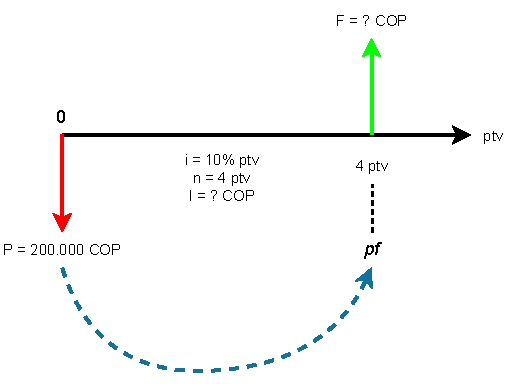
\includegraphics[trim=-5 -5 -5 -5 , scale=1]{2_Capitulo/ejemplos/1/Capitulo2Ejercicio1a2_v2.pdf} }                                         \\ \hline
    %%%%%%%%%%%%% FIN INSERCIÓN DE IMAGEN
    %%%%%FIN FLUJO DE CAJA

    %%%%% INICIO DECLARACIÓN FORMULAS
    %%%%%%%%%%% INICIO TITULO
    \rowcolor[HTML]{FFB183}
    \multicolumn{3}{|c|}{\cellcolor[HTML]{FFB183}\textbf{4. Declaración de fórmulas}}                                                                            \\ \hline
    %%%%%%%%%%% FIN TITULO
    %%%%%%%%%%% INICIO MATEMÁTICAS

    $I = Pin\hspace{0.3cm} \textit{Interés monetario simple}$ & \multicolumn{2}{c|}{$F = P + I \hspace{0.3cm} \textit{Valor futuro}$}                            \\ \hline
    %%%%%%%%%% FIN MATEMÁTICAS
    %%%%%% INICIO DESARROLLO MATEMÁTICO
    \rowcolor[HTML]{FFB183}
    %%%%%%%%%%INICIO TITULO
    \multicolumn{3}{|c|}{\cellcolor[HTML]{FFB183}\textbf{5. Desarrollo matemático}}                                                                              \\ \hline
    %%%%%%%%%% FIN TITULO
    %%%%%%%%%% INICIO MATEMÁTICAS
    $n=4ptv$                                                  & \multicolumn{2}{c|}{}                                                                            \\ $I_{1}= 200{.}000$ COP$\cdot0.1\cdot1$ & \multicolumn{2}{c|}{$F =  200{.}000$ COP + $20{.}000$ COP + $22{.}000$ COP}  \\ $I_{1}=  20{.}000$ COP & \multicolumn{2}{c|}{$+ 24{.}200$ COP + $26{.}620$ COP}  \\
    $I_{2}= 220{.}000\cdot0.1\cdot1$ COP   & \multicolumn{2}{c|}{$F= P+I$} \\
    $I_{2}= 22{.}000$ COP                  & \multicolumn{2}{c|}{$F=200{.}000$ COP$+92{.}820$ COP}   \\
    $I_{3}= 242{.}000\cdot0.1\cdot1$ COP   & \multicolumn{2}{c|}{$F= 292{.}820$ COP}                \\
    $I_{3}= 24{.}200$ COP                  & \multicolumn{2}{c|}{}                                                           \\
    $I_{4}= 266{.}200\cdot0.1\cdot1$ COP   & \multicolumn{2}{c|}{}                                                                            \\
    $I_{4}= 26{.}620$ COP                  & \multicolumn{2}{c|}{}                                                                            \\
    $I= 20{.}000 COP + 22{.}000 COP + 24{.}200 COP + 26{.}620 COP$& \multicolumn{2}{c|}{}                                        \\
    $I= 92{.}820$ COP                      & \multicolumn{2}{c|}{}
    
    \\ \hline
    %%%%%%%%%% FIN MATEMÁTICAS
    %%%%%% FIN DESARROLLO MATEMÁTICO
    %%%%%% INICIO RESPUESTA
    \rowcolor[HTML]{FFB183}
    %%%%%%%%%%INICIO TITULO
    \multicolumn{3}{|c|}{\cellcolor[HTML]{FFB183}\textbf{6. Respuesta}}                                                                                          \\ \hline
    %%%%%%%%%% FIN TITULO
    %%%%%%%%%% INICIO RESPUESTA MATEMÁTICA
    $I= 92{.}820 COP$                                         &
    \multicolumn{2}{c|}{$F= 292{.}820 COP$
    }                                                                                                                                                            \\ \hline
    %%%%%%%%%% FIN MATEMÁTICAS
    %%%%%% FIN RESPUESTA
  \end{longtable}
  %Se crean dos lineas en blanco para que no quede el siguiente texto tan pegado
  %\newline \newline %USARLO SI CREES QUE ES NECESARIO
\end{center}
%%%%%%%%%%%%%%%%%%%%%%%%%%FIN EJERCICIO 1 %%%%%%%%%%%%%%%%%%%%%%%%%%%



Representando en una tabla la información obtenida en el apartado anterior del ejercicio se tiene lo siguiente:\\

\begin{table}[htbp]
   \begin{center}
      \begin{tabular}{|l|l|l|l|}
         \hline
         Período & Capital Inicial & Interés     & Capital Final \\
         \hline
         0 & 200.000 COP & 0 COP      & 200.000 COP \\ \hline
         1 & 200.000 COP & 20.000 COP & 220.000 COP \\ \hline
         2 & 220.000 COP & 22.000 COP & 242.000 COP \\ \hline
         3 & 242.000 COP & 24.200 COP & 266.000 COP \\ \hline
         4 & 266.000 COP & 26.000 COP & 292.000 COP \\ \hline
      \end{tabular}
      \label{tabla:interesCompuesto1}
   \end{center}
\end{table}
\textbf{Generalizando:}\\
\begin{table}[htbp]
   \begin{center}
      \begin{tabular}{|l|l|l|l|}
         \hline
         Período & Capital Inicial & Interés         & Capital Final                                       \\
         \hline
         0       & P               & 0               & $F_{0}$=P                                           \\ \hline
         1       & P               & Pi              & $F_{1}$ = P + Pi = P(1+i)                           \\ \hline
         2       & P(1+i)          & P(1+i)i         & $F_{2}$ = P(1+i) + P(1+i)i = $P(1+i)^{2}$           \\ \hline
         .       & .               & .               & .                                                   \\ \hline
         ..      & ..              & ..              & ..                                                  \\ \hline
         ...     & ...             & ...             & ...                                                 \\ \hline
         n       & $P(1+i)^{n-1}$  & $P(1+i)^{n-1}i$ & $F_{n} = P(1+i)^{n-1} + P(1+i)^{n-1}i = P(1+i)^{n}$ \\ \hline
      \end{tabular}
      \label{tabla:interesCompuesto2}
   \end{center}
\end{table}

Se concluye que la fórmula del interés compuesto es:\\
$F = P(1+i)^n$ \hspace{20 pt} \textit{Valor futuro}\\

\textbf{Volviendo al ejemplo 1:}\\
$F = P(1+i)^n$\\
$F =  200.000 (1+0,1)^4$ COP\\
$F =  292.820$ COP\\

%%%%%%%%%% NO OLVIDAR COLOCAR ESTE COMENTARIO CON EL NUMERO DE EJERCICIO %%%%%%%%%%%%%
%%%%%%%%%%%%%%%%%%% EJERCICIO 2 %%%%%%
%%Text bf para negrilla , el \\ es para el salto de linea.
%%El primer \\ hace un espacio en el texto y el 2 \\ crea otro espacio
\textbf{Ejemplo 2}\newline
El jefe de producción de una fábrica debe decidir entre dos máquinas A y B. Las características de cada una son: \\
\begin{center}
		\begin{tabular}{|p{1cm}|p{2cm}|p{2cm}|p{2cm}|p{3cm}|}
			\hline
			\rowcolor{white!50}
			\textbf{Maq.} & \textbf{C} & \textbf{K} & \textbf{S} & \textbf{CAO} \\ \hline
			A            & 800.000 COP   & 3 años     & 200.000 COP    & 25.000 COP       \\ \hline
			B            & 600.000 COP   & 2 años     & 150.000 COP    & 30.000 COP       \\ \hline
		\end{tabular}
\end{center}

Con una tasa del 36\% nominal anual año vencido, determinar la mejor alternativa.

\textbf{Solución.}\\
\begin{center}
	\renewcommand{\arraystretch}{1.5}% Margenes de las celdas
	%Creación de la cuadricula
	\begin{longtable}[H]{|c|c|c|}
		%Creamos una linea horizontal
		\hline
		%Definimos el color de la primera fila
		\rowcolor[HTML]{FFB183}
		%%%%% INICIO ASIGNACIÓN FECHA FOCAL %%%%%%%
		%%%%%%%%%% INICIO TITULO
		%Lo que se hace aquí es mezclar las 3 columnas en una sola
		\multicolumn{3}{|c|}{\cellcolor[HTML]{FFB183}\textbf{1. Asignación período focal}}   \\ \hline
		%%%%%%%%%% FIN TITULO
		%%%%% INICIO DECLARACIÓN DE VARIABLES %%%%%%%
		\multicolumn{3}{|c|}{$pf = 0  \textit{ pav }$} \\ \hline
		%Definimos el color de la primera fila
		\rowcolor[HTML]{FFB183}
		%%%%% INICIO DECLARACIÓN DE VARIABLES %%%%%%%
		%%%%%%%%%% INICIO TITULO
		\multicolumn{3}{|c|}{\cellcolor[HTML]{FFB183}\textbf{2. Declaración de variables}}                                                                                   \\ \hline
		%%%%%%%%%% FIN TITULO
		%%%%%%%%%% INICIO DE MATEMÁTICAS
		$\text{Alternativa A}$ & $\text{Alternativa B}$ & $i= 36\% \text{ pav }$\\
		$C =  800{.}000\text{ COP}$ & $C =  600{.}000\text{ COP}$ & $CPUE =  ?\text{ COP}$\\
		$K =  3 \textit{ años}$ & $K =  2 \textit{ años}$ & \\
		$S =  200{.}000\text{ COP}$ & $S =  150{.}000\text{ COP}$ & \\
		$CAO =  25{.}000\text{ COP}$ & $CAO =  30{.}000\text{ COP}$ & \\
 		$n_{1}= 3 \text{ pav}$ & $n_{2}= 2 \text{ pav}$ &   \\\hline 
		%%%%%%%%%% FIN DE MATEMÁTICAS
		%%%%% FIN DECLARACIÓN DE VARIABLES


		%%%%% INICIO FLUJO DE CAJA
		\rowcolor[HTML]{FFB183}
		\multicolumn{3}{|c|}{\cellcolor[HTML]{FFB183}\textbf{3. Diagrama de flujo de caja}}\\ \hline
		%Mezclamos 3 columnas y pondremos el dibujo
		%%%%%%%%%%%%% INSERCIÓN DE LA IMAGEN
		\multicolumn{3}{|c|}{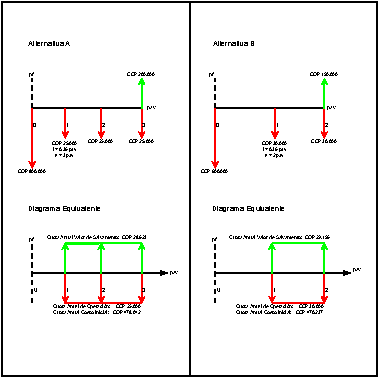
\includegraphics[trim=-5 -5 -5 -5 , scale=2]{10_Capitulo/ejemplos/2/Ejemplo_2.pdf}}
        \\\hline
		%%%%%%%%%%%%% FIN INSERCIÓN DE IMAGEN
		%%%%%FIN FLUJO DE CAJA



		%%%%% INICIO DECLARACIÓN FORMULAS
		%%%%%%%%%%% INICIO TITULO
		\rowcolor[HTML]{FFB183}
		\multicolumn{3}{|c|}{\cellcolor[HTML]{FFB183}\textbf{4. Declaración de fórmulas}} \\ \hline
		%%%%%%%%%%% FIN TITULO
		%%%%%%%%%%% INICIO MATEMÁTICAS

		\multicolumn{3}{|c|}{$VP=R\frac{1-(1+i_{1})^{-n}}{i_{2}} \text{ Valor presente serie uniforme vencida}$}\\ 
		\multicolumn{3}{|c|}{$VF=R\frac{1-(1+i_{1})^{n}}{i_{2}} \text{ Valor futuro aserie uniforme vencida}$}\\\hline
		%%%%%%%%%% FIN MATEMÁTICAS
		%%%%%% INICIO DESARROLLO MATEMÁTICO
		\rowcolor[HTML]{FFB183}
		%%%%%%%%%%INICIO TITULO
		\multicolumn{3}{|c|}{\cellcolor[HTML]{FFB183}\textbf{5. Desarrollo matemático}}   \\ \hline
		%%%%%%%%%% FIN TITULO
		%%%%%%%%%% INICIO MATEMÁTICAS
		Alternativa A & \multicolumn{2}{c|}{Alternativa B}\\ \hline
		Cuota anual costo inicial & \multicolumn{2}{c|}{Cuota anual costo inicial} \\
		${R=\frac{800{.}000}{\frac{1-(1,36)^{-3}}{0,36}} = 178{.}042}\text{ COP}$ & \multicolumn{2}{c|}{${R=\frac{600{.}000}{\frac{1-(1,36)^{-2}}{0,36}} = 470{.}237 }\text{ COP}$} \\
		Cuota anual valor salvamento & \multicolumn{2}{c|}{Cuota anual valor salvamento}\\
		$R=\frac{200{.}000}{\frac{(1,36)^{3}}{0,36}} = 28{.}623\text{ COP} $ & \multicolumn{2}{c|}{$R=\frac{150{.}000}{\frac{(1,36)^{2}}{0,36}} = 29{.}196 \text{ COP}$} \\
		CPUE alternativa A & \multicolumn{2}{c|}{CPUE alternativa B} \\ 
		$CPUE_{A} = 28.623-478.042-25.000 $ & \multicolumn{2}{c|}{$CPUE_{B} = 29.196-470.237-30.000$}\\ 
		$CPUE_{A} = -474.419\text{ COP}$ & \multicolumn{2}{c|}{$CPUE_{B} = -471.04$\text{ COP}}\\
		\hline
		%%%%%%%%%% FIN MATEMÁTICAS
		%%%%%% FIN DESARROLLO MATEMÁTICO

		\rowcolor[HTML]{FFB183}
		\multicolumn{3}{|c|}{\cellcolor[HTML]{FFB183}\textbf{6. Respuesta}}    \\ \hline

		\multicolumn{3}{|c|}{La alternativa que representa menores perdidad es la B.} \\ 
		\hline
	\end{longtable}
	%Se crean dos lineas en blanco para que no quede el siguiente texto tan pegado
	%\newline \newline
\end{center}
%%%%%%%%%%%%%%%%%%%%%%%%%%FIN EJERCICIO X %%%%%%%%%%%%%%%%%%%%%%%%%%%




\section{Tasa de interés nominal anual (j)}
Corresponde a la anualización de la tasa periódica (i):\\
$j = i(m)$\\
%%%%%%%%%% NO OLVIDAR COLOCAR ESTE COMENTARIO CON EL NUMERO DE EJERCICIO %%%%%%%%%%%%%
%%%%%%%%%%%%%%%%%%% EJERCICIO 2 %%%%%%
%%Text bf para negrilla , el \\ es para el salto de linea.
%%El primer \\ hace un espacio en el texto y el 2 \\ crea otro espacio
\textbf{Ejemplo 2}\newline
El jefe de producción de una fábrica debe decidir entre dos máquinas A y B. Las características de cada una son: \\
\begin{center}
		\begin{tabular}{|p{1cm}|p{2cm}|p{2cm}|p{2cm}|p{3cm}|}
			\hline
			\rowcolor{white!50}
			\textbf{Maq.} & \textbf{C} & \textbf{K} & \textbf{S} & \textbf{CAO} \\ \hline
			A            & 800.000 COP   & 3 años     & 200.000 COP    & 25.000 COP       \\ \hline
			B            & 600.000 COP   & 2 años     & 150.000 COP    & 30.000 COP       \\ \hline
		\end{tabular}
\end{center}

Con una tasa del 36\% nominal anual año vencido, determinar la mejor alternativa.

\textbf{Solución.}\\
\begin{center}
	\renewcommand{\arraystretch}{1.5}% Margenes de las celdas
	%Creación de la cuadricula
	\begin{longtable}[H]{|c|c|c|}
		%Creamos una linea horizontal
		\hline
		%Definimos el color de la primera fila
		\rowcolor[HTML]{FFB183}
		%%%%% INICIO ASIGNACIÓN FECHA FOCAL %%%%%%%
		%%%%%%%%%% INICIO TITULO
		%Lo que se hace aquí es mezclar las 3 columnas en una sola
		\multicolumn{3}{|c|}{\cellcolor[HTML]{FFB183}\textbf{1. Asignación período focal}}   \\ \hline
		%%%%%%%%%% FIN TITULO
		%%%%% INICIO DECLARACIÓN DE VARIABLES %%%%%%%
		\multicolumn{3}{|c|}{$pf = 0  \textit{ pav }$} \\ \hline
		%Definimos el color de la primera fila
		\rowcolor[HTML]{FFB183}
		%%%%% INICIO DECLARACIÓN DE VARIABLES %%%%%%%
		%%%%%%%%%% INICIO TITULO
		\multicolumn{3}{|c|}{\cellcolor[HTML]{FFB183}\textbf{2. Declaración de variables}}                                                                                   \\ \hline
		%%%%%%%%%% FIN TITULO
		%%%%%%%%%% INICIO DE MATEMÁTICAS
		$\text{Alternativa A}$ & $\text{Alternativa B}$ & $i= 36\% \text{ pav }$\\
		$C =  800{.}000\text{ COP}$ & $C =  600{.}000\text{ COP}$ & $CPUE =  ?\text{ COP}$\\
		$K =  3 \textit{ años}$ & $K =  2 \textit{ años}$ & \\
		$S =  200{.}000\text{ COP}$ & $S =  150{.}000\text{ COP}$ & \\
		$CAO =  25{.}000\text{ COP}$ & $CAO =  30{.}000\text{ COP}$ & \\
 		$n_{1}= 3 \text{ pav}$ & $n_{2}= 2 \text{ pav}$ &   \\\hline 
		%%%%%%%%%% FIN DE MATEMÁTICAS
		%%%%% FIN DECLARACIÓN DE VARIABLES


		%%%%% INICIO FLUJO DE CAJA
		\rowcolor[HTML]{FFB183}
		\multicolumn{3}{|c|}{\cellcolor[HTML]{FFB183}\textbf{3. Diagrama de flujo de caja}}\\ \hline
		%Mezclamos 3 columnas y pondremos el dibujo
		%%%%%%%%%%%%% INSERCIÓN DE LA IMAGEN
		\multicolumn{3}{|c|}{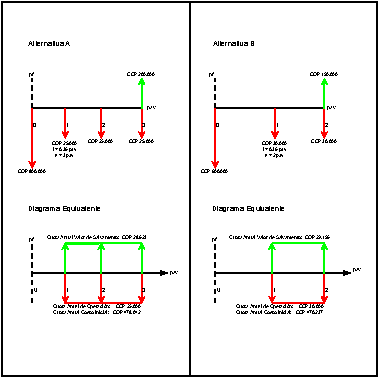
\includegraphics[trim=-5 -5 -5 -5 , scale=2]{10_Capitulo/ejemplos/2/Ejemplo_2.pdf}}
        \\\hline
		%%%%%%%%%%%%% FIN INSERCIÓN DE IMAGEN
		%%%%%FIN FLUJO DE CAJA



		%%%%% INICIO DECLARACIÓN FORMULAS
		%%%%%%%%%%% INICIO TITULO
		\rowcolor[HTML]{FFB183}
		\multicolumn{3}{|c|}{\cellcolor[HTML]{FFB183}\textbf{4. Declaración de fórmulas}} \\ \hline
		%%%%%%%%%%% FIN TITULO
		%%%%%%%%%%% INICIO MATEMÁTICAS

		\multicolumn{3}{|c|}{$VP=R\frac{1-(1+i_{1})^{-n}}{i_{2}} \text{ Valor presente serie uniforme vencida}$}\\ 
		\multicolumn{3}{|c|}{$VF=R\frac{1-(1+i_{1})^{n}}{i_{2}} \text{ Valor futuro aserie uniforme vencida}$}\\\hline
		%%%%%%%%%% FIN MATEMÁTICAS
		%%%%%% INICIO DESARROLLO MATEMÁTICO
		\rowcolor[HTML]{FFB183}
		%%%%%%%%%%INICIO TITULO
		\multicolumn{3}{|c|}{\cellcolor[HTML]{FFB183}\textbf{5. Desarrollo matemático}}   \\ \hline
		%%%%%%%%%% FIN TITULO
		%%%%%%%%%% INICIO MATEMÁTICAS
		Alternativa A & \multicolumn{2}{c|}{Alternativa B}\\ \hline
		Cuota anual costo inicial & \multicolumn{2}{c|}{Cuota anual costo inicial} \\
		${R=\frac{800{.}000}{\frac{1-(1,36)^{-3}}{0,36}} = 178{.}042}\text{ COP}$ & \multicolumn{2}{c|}{${R=\frac{600{.}000}{\frac{1-(1,36)^{-2}}{0,36}} = 470{.}237 }\text{ COP}$} \\
		Cuota anual valor salvamento & \multicolumn{2}{c|}{Cuota anual valor salvamento}\\
		$R=\frac{200{.}000}{\frac{(1,36)^{3}}{0,36}} = 28{.}623\text{ COP} $ & \multicolumn{2}{c|}{$R=\frac{150{.}000}{\frac{(1,36)^{2}}{0,36}} = 29{.}196 \text{ COP}$} \\
		CPUE alternativa A & \multicolumn{2}{c|}{CPUE alternativa B} \\ 
		$CPUE_{A} = 28.623-478.042-25.000 $ & \multicolumn{2}{c|}{$CPUE_{B} = 29.196-470.237-30.000$}\\ 
		$CPUE_{A} = -474.419\text{ COP}$ & \multicolumn{2}{c|}{$CPUE_{B} = -471.04$\text{ COP}}\\
		\hline
		%%%%%%%%%% FIN MATEMÁTICAS
		%%%%%% FIN DESARROLLO MATEMÁTICO

		\rowcolor[HTML]{FFB183}
		\multicolumn{3}{|c|}{\cellcolor[HTML]{FFB183}\textbf{6. Respuesta}}    \\ \hline

		\multicolumn{3}{|c|}{La alternativa que representa menores perdidad es la B.} \\ 
		\hline
	\end{longtable}
	%Se crean dos lineas en blanco para que no quede el siguiente texto tan pegado
	%\newline \newline
\end{center}
%%%%%%%%%%%%%%%%%%%%%%%%%%FIN EJERCICIO X %%%%%%%%%%%%%%%%%%%%%%%%%%%



\textbf{Ejemplo 3}\\
Hallar el valor presente de la siguiente serie con una tasa del 5\% periodo anual mes vencido, utilizando dos formas para resolverlo.\\

%imagen 4
\begin{center}
	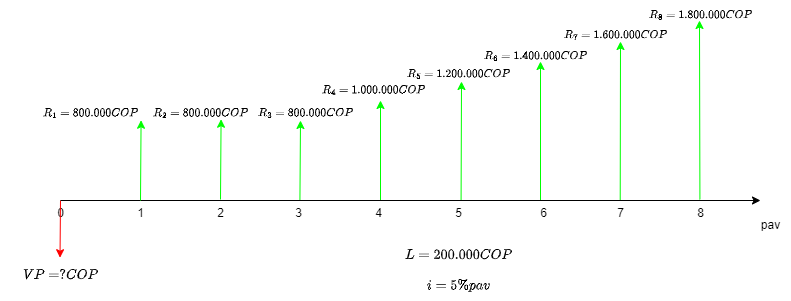
\includegraphics[height=4.0cm]{6_Capitulo/img/ejemplos/6_5}
\end{center}

\textbf{Solución:}

\begin{center}
	\textbf{Primera forma:}
\end{center}

%La tabla ira centrada
\begin{center}
	\renewcommand{\arraystretch}{1.4}% Margenes de las celdas
	%Creación de la cuadricula de 3 columnas
	\begin{longtable}[H]{|c|c|c|}
		%Creamos una linea horizontal
		\hline
		%Definimos el color de la primera fila
		\rowcolor[HTML]{FFB183}
		%%%%% INICIO ASIGNACIÓN PERIODO FOCAL %%%%%%%
		%%%%%%%%%% INICIO TITULO
		%Lo que se hace aquí es mezclar las 3 columnas en una sola
		\multicolumn{3}{|c|}{\cellcolor[HTML]{FFB183}\textbf{1. Asignación período focal}}                                                                                                                            \\ \hline
		\multicolumn{3}{|c|}{$Pf=0 \textit{ pav}$}                                                                                                                                                                    \\ \hline
		%%%%%%%%%% FIN TITULO
		%%%%% INICIO DECLARACIÓN DE VARIABLES %%%%%%%
		%%%%%%%%%% INICIO TITULO
		%Lo que se hace aquí es mezclar las 3 columnas en una sola
		\multicolumn{3}{|c|}{\cellcolor[HTML]{FFB183}\textbf{2. Declaración de variables}}                                                                                                                            \\ \hline
		%%%%%%%%%% FIN TITULO
		%%%%%%%%%% INICIO DE MATEMÁTICAS
		%Cada & hace referencia al paso de la siguiente columna
		\multicolumn{2}{|c|}{$\hspace{2 cm}R=800{.}000 COP \hspace{2 cm}$} & $i=5\%\textit{ pav}$                                                                                                                     \\
		\multicolumn{2}{|c|}{$L=  200{.}000COP$}                           & $n_1=2\textit{ pav}$                                                                                                                     \\
		\multicolumn{2}{|c|}{$VP= ?COP $}                                  & $n_2=6\textit{ pav}$                                                                                                                     \\\hline

		%%%%%%%%%% FIN DE MATEMÁTICAS
		%%%%% FIN DECLARACIÓN DE VARIABLES


		%%%%% INICIO FLUJO DE CAJA
		\rowcolor[HTML]{FFB183}
		\multicolumn{3}{|c|}{\cellcolor[HTML]{FFB183}\textbf{3. Diagrama de flujo de caja}}                                                                                                                           \\ \hline
		%Mezclamos 3 columnas y pondremos el dibujo
		%%%%%%%%%%%%% INSERCIÓN DE LA IMAGEN
		%Deberán descargar las imágenes respectivas del drive y pegarlas en la carpeta
		%n_capitulo/img/ejemplos/1/capitulo1ejemplo1.pdf  (el /1/ es el numero del ejemplo)
		\multicolumn{3}{|c|}{ 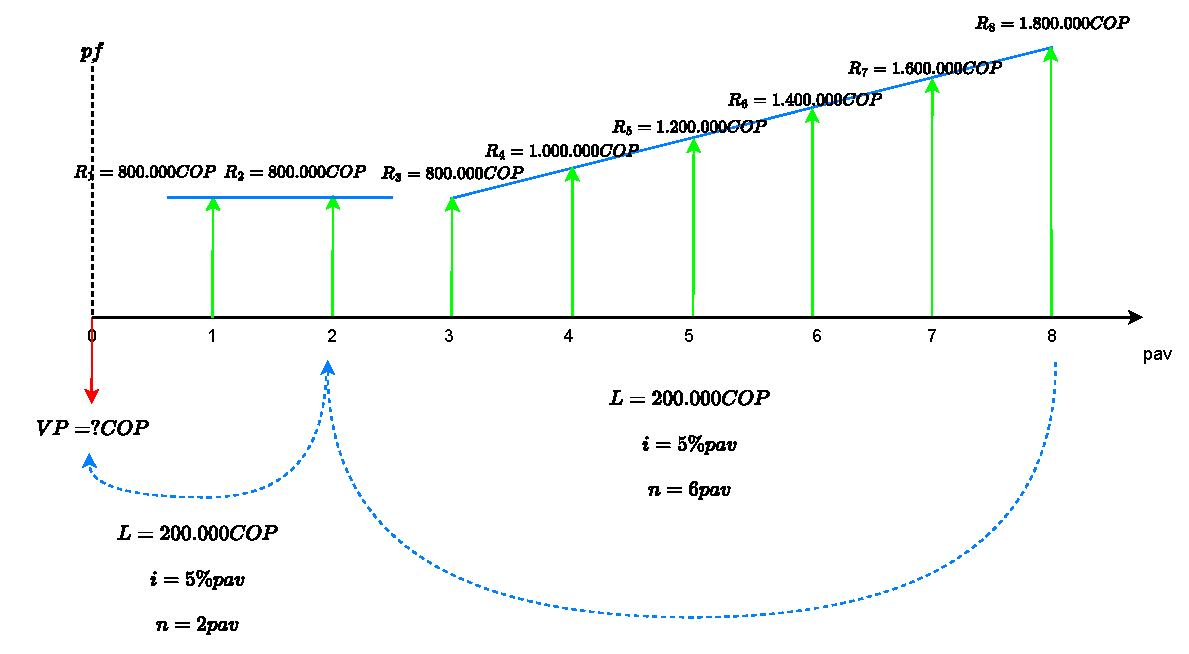
\includegraphics[trim=-5 -5 -5 -5 , scale=0.4]{6_Capitulo/ejemplos/3/Capitulo6Ejemplo3a.pdf} }

		\\ \hline
		%%%%%%%%%%%%% FIN INSERCIÓN DE IMAGEN
		%%%%%FIN FLUJO DE CAJA

		%%%%% INICIO DECLARACIÓN FORMULAS
		%%%%%%%%%%% INICIO TITULO
		\rowcolor[HTML]{FFB183}
		\multicolumn{3}{|c|}{\cellcolor[HTML]{FFB183}\textbf{4. Declaración de fórmulas}}                                                                                                                             \\ \hline
		%%%%%%%%%%% FIN TITULO
		%%%%%%%%%%% INICIO MATEMÁTICAS

		\multicolumn{3}{|c|}{$VP=R(\frac{1-(1+i)^{-n}}{i})+\frac{L}{i}[\frac{1-(1+i)^{-n}}{i}-n(1+i)^{-n}] \hspace{0.4 cm} \textit{Valor presente gradiente aritmético}$}                                             \\
		\multicolumn{3}{|c|}{$VP=R(\frac{1-(1+i)^{-n}}{i}) \hspace{0.4 cm} \textit{Valor presente de una serie unifrome vencida}$}                                                                                    \\
		\multicolumn{3}{|c|}{$P=F(1+i)^{-n} \hspace{0.4 cm} \textit{Valor presente dado un valor futuro}$}                                                                                                            \\ \hline

		%%%%%%%%%% FIN MATEMÁTICAS
		%%%%%% INICIO DESARROLLO MATEMÁTICO
		\rowcolor[HTML]{FFB183}
		%%%%%%%%%%INICIO TITULO
		\multicolumn{3}{|c|}{\cellcolor[HTML]{FFB183}\textbf{5. Desarrollo matemático}}                                                                                                                               \\ \hline
		%%%%%%%%%% FIN TITULO
		%%%%%%%%%% INICIO MATEMÁTICAS
		\multicolumn{3}{|c|}{$VP=  800{.}000COP(\frac{1-(1+0.05)^{-2}}{0.05})+[  800{.}000COP(\frac{1-(1+0.05)^{-6}}{0.05})+\frac{ COP 200{.}000}{0.05}[\frac{1-(1+0.05)^{-6}}{0.05}-6(1+0.05)^{-6}]]$} \\
		\multicolumn{3}{|c|}{$*(1+0.05)^{-2}$}\\
		\multicolumn{3}{|c|}{$VP= 7{.}341{.} \textit{  COP }$}                                                                                                                                                       \\ \hline


		%%%%%%%%%% FIN MATEMÁTICAS
		%%%%%% FIN DESARROLLO MATEMÁTICO
		%%%%%% INICIO RESPUESTA
		\rowcolor[HTML]{FFB183}
		%%%%%%%%%%INICIO TITULO
		\multicolumn{3}{|c|}{\cellcolor[HTML]{FFB183}\textbf{6. Respuesta}}                                                                                                                                           \\ \hline
		%%%%%%%%%% FIN TITULO
		%%%%%%%%%% INICIO RESPUESTA MATEMÁTICA
		\multicolumn{3}{|c|}{\textbf{$\textit{VP= 7{.}341{.}634.83  COP }$}}
		\\ \hline
		%%%%%%%%%% FIN MATEMÁTICAS
		%%%%%% FIN RESPUESTA
	\end{longtable}
	%Se crean dos lineas en blanco para que no quede el siguiente texto tan pegado
	%\newline \newline %USARLO SI CREES QUE ES NECESARIO
\end{center}
%%%%%%%%%%%%%%%%%%%%%%%%%%FIN EJERCICIO 3.1 %%%%%%%%%%%%%%%%%%%%%%%%%%%

\textbf{Segunda forma:}


%La tabla ira centrada
\begin{center}
	\renewcommand{\arraystretch}{1.4}% Margenes de las celdas
	%Creación de la cuadricula de 3 columnas
	\begin{longtable}[H]{|c|c|c|}
		%Creamos una linea horizontal
		\hline
		%Definimos el color de la primera fila
		\rowcolor[HTML]{FFB183}
		%%%%% INICIO ASIGNACIÓN PERIODO FOCAL %%%%%%%
		%%%%%%%%%% INICIO TITULO
		%Lo que se hace aquí es mezclar las 3 columnas en una sola
		\multicolumn{3}{|c|}{\cellcolor[HTML]{FFB183}\textbf{1. Asignación período focal}}                                                                                                                                                            \\ \hline
		\multicolumn{3}{|c|}{$pf=0 \textit{ pav}$}                                                                                                                                                                                                    \\ \hline
		%%%%%%%%%% FIN TITULO
		%%%%% INICIO DECLARACIÓN DE VARIABLES %%%%%%%
		%%%%%%%%%% INICIO TITULO
		%Lo que se hace aquí es mezclar las 3 columnas en una sola
		\multicolumn{3}{|c|}{\cellcolor[HTML]{FFB183}\textbf{2. Declaración de variables}}                                                                                                                                                            \\ \hline
		%%%%%%%%%% FIN TITULO
		%%%%%%%%%% INICIO DE MATEMÁTICAS
		%Cada & hace referencia al paso de la siguiente columna
		\multicolumn{2}{|c|}{$\hspace{2 cm}R=  800{.}000COP\hspace{2 cm}$} & $i=5\%\textit{ pav}$                                                                                                                                                     \\
		\multicolumn{2}{|c|}{$L=  200{.}000COP$}                           & $n_1=3\textit{ pav}$                                                                                                                                                     \\
		\multicolumn{2}{|c|}{$VP=? COP $}                                  & $n_2=5\textit{ pav}$                                                                                                                                                     \\\hline

		%%%%%%%%%% FIN DE MATEMÁTICAS
		%%%%% FIN DECLARACIÓN DE VARIABLES


		%%%%% INICIO FLUJO DE CAJA
		\rowcolor[HTML]{FFB183}
		\multicolumn{3}{|c|}{\cellcolor[HTML]{FFB183}\textbf{3. Diagrama de flujo de caja}}                                                                                                                                                           \\ \hline
		%Mezclamos 3 columnas y pondremos el dibujo
		%%%%%%%%%%%%% INSERCIÓN DE LA IMAGEN
		%Deberán descargar las imágenes respectivas del drive y pegarlas en la carpeta
		%n_capitulo/img/ejemplos/1/capitulo1ejemplo1.pdf  (el /1/ es el numero del ejemplo)
		\multicolumn{3}{|c|}{ 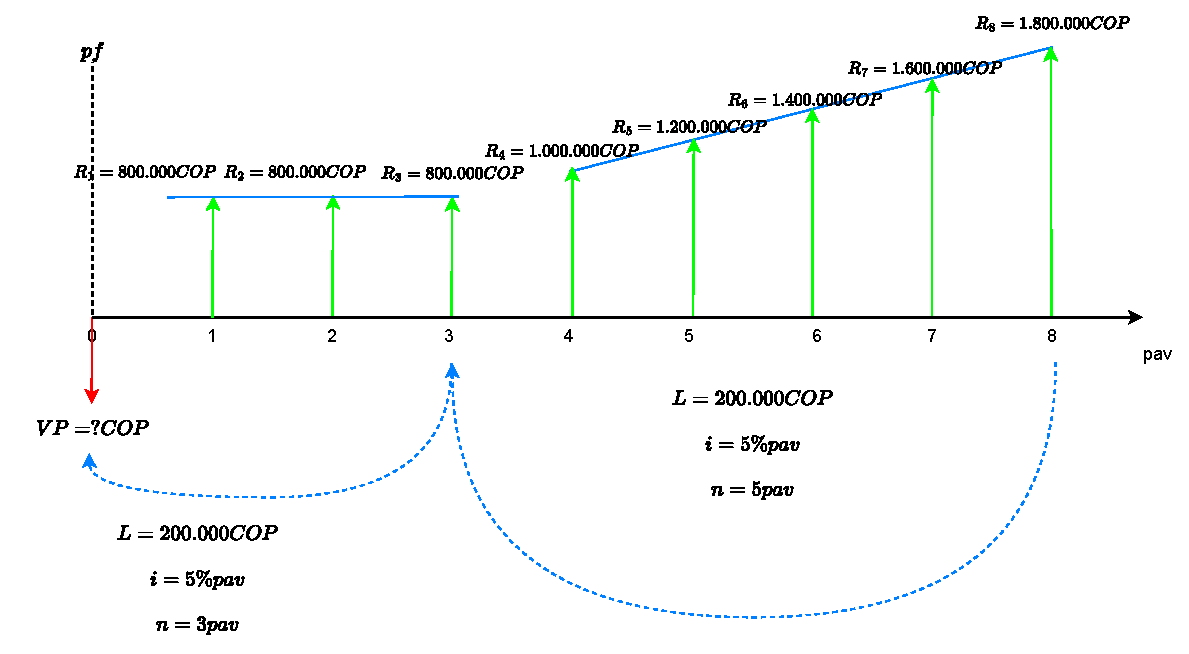
\includegraphics[trim=-5 -5 -5 -5 , scale=0.4]{6_Capitulo/ejemplos/3/Capitulo6Ejemplo3b.pdf} }

		\\ \hline
		%%%%%%%%%%%%% FIN INSERCIÓN DE IMAGEN
		%%%%%FIN FLUJO DE CAJA

		%%%%% INICIO DECLARACIÓN FORMULAS
		%%%%%%%%%%% INICIO TITULO
		\rowcolor[HTML]{FFB183}
		\multicolumn{3}{|c|}{\cellcolor[HTML]{FFB183}\textbf{4. Declaración de fórmulas}}                                                                                                                                                             \\ \hline
		%%%%%%%%%%% FIN TITULO
		%%%%%%%%%%% INICIO MATEMÁTICAS

		\multicolumn{3}{|c|}{$VP=R(\frac{1-(1+i)^{-n}}{i})+\frac{L}{i}[\frac{1-(1+i)^{-n}}{i}-n(1+i)^{-n}] \hspace{0.4 cm} \textit{Valor presente gradiente aritmético}$}                                                                             \\
		\multicolumn{3}{|c|}{$VP=R(\frac{1-(1+i)^{-n}}{i}) \hspace{0.4 cm} \textit{Valor presente de una serie unifrome vencida}$}                                                                                                                    \\
		\multicolumn{3}{|c|}{$P=F(1+i)^{-n} \hspace{0.4 cm} \textit{Valor presente dado un valor futuro}$}                                                                                                                                            \\ \hline

		%%%%%%%%%% FIN MATEMÁTICAS
		%%%%%% INICIO DESARROLLO MATEMÁTICO
		\rowcolor[HTML]{FFB183}
		%%%%%%%%%%INICIO TITULO
		\multicolumn{3}{|c|}{\cellcolor[HTML]{FFB183}\textbf{5. Desarrollo matemático}}                                                                                                                                                               \\ \hline
		%%%%%%%%%% FIN TITULO
		%%%%%%%%%% INICIO MATEMÁTICAS
		\multicolumn{3}{|c|}{$VP=  800{.}000COP(\frac{1-(1+0.05)^{-3}}{0.05})+[  1{.}000{.}000COP(\frac{1-(1+0.05)^{-5}}{0.05})+\frac{  200{.}000COP}{0.05}[\frac{1-(1+0.05)^{-5}}{0.05}-6(1+0.05)^{-6}]]$} \\
		\multicolumn{3}{|c|}{$*(1+0.05)^{-3}\hspace{0.2 cm}\textit{Ec. eqv.}$}\\
		\multicolumn{3}{|c|}{$VP= 7{.}341{.}634 \textit{  COP }$}                                                                                                                                                                                       \\ \hline


		%%%%%%%%%% FIN MATEMÁTICAS
		%%%%%% FIN DESARROLLO MATEMÁTICO
		%%%%%% INICIO RESPUESTA
		\rowcolor[HTML]{FFB183}
		%%%%%%%%%%INICIO TITULO
		\multicolumn{3}{|c|}{\cellcolor[HTML]{FFB183}\textbf{6. Respuesta}}                                                                                                                                                                           \\ \hline
		%%%%%%%%%% FIN TITULO
		%%%%%%%%%% INICIO RESPUESTA MATEMÁTICA
		\multicolumn{3}{|c|}{{$\textit{El valor presente de la serie es  7{.}341{.}634 COP }$}}
		\\ \hline
		%%%%%%%%%% FIN MATEMÁTICAS
		%%%%%% FIN RESPUESTA
	\end{longtable}
	%Se crean dos lineas en blanco para que no quede el siguiente texto tan pegado
	%\newline \newline %USARLO SI CREES QUE ES NECESARIO
\end{center}
%%%%%%%%%%%%%%%%%%%%%%%%%%FIN EJERCICIO 3.2 %%%%%%%%%%%%%%%%%%%%%%%%%%%



\section{Equivalencia de tasas ($i_{1} \equiv i_{2}$)}
Las tasas equivalentes de interés,  son aquellas que teniendo diferente periodicidad y/o 
modalidad de liquidación de intereses producen el mismo monto al final o al comienzo del flujo.\\
\\
\textbf{Ejemplo 4}\\
	Hallar el monto del siguiente flujo de caja que renta una tasa del 15\% periódica año vencido. \\
	\\
	%imagen 5
	\begin{center}
		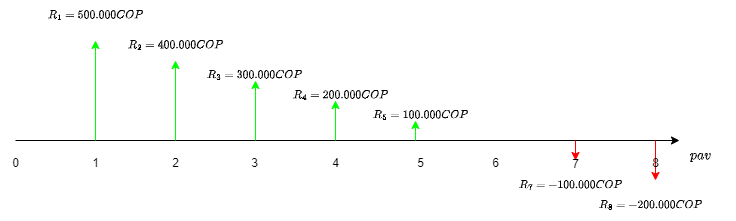
\includegraphics[height=4.5cm]{6_Capitulo/img/ejemplos/6_6}
	\end{center}
	
	\textbf{Solución:}
	
		%La tabla ira centrada
	\begin{center}
		\renewcommand{\arraystretch}{1.4}% Margenes de las celdas
		%Creación de la cuadricula de 3 columnas
		\begin{longtable}[H]{|c|c|c|}
			%Creamos una linea horizontal
			\hline
			%Definimos el color de la primera fila
			\rowcolor[HTML]{FFB183}
			%%%%% INICIO ASIGNACIÓN PERIODO FOCAL %%%%%%%
			%%%%%%%%%% INICIO TITULO
			%Lo que se hace aquí es mezclar las 3 columnas en una sola
			\multicolumn{3}{|c|}{\cellcolor[HTML]{FFB183}\textbf{1. Asignación período focal}}  \\ \hline
			\multicolumn{3}{|c|}{$pf=8 \textit{ pav}$} \\ \hline
			%%%%%%%%%% FIN TITULO
			%%%%% INICIO DECLARACIÓN DE VARIABLES %%%%%%%
			%%%%%%%%%% INICIO TITULO
			%Lo que se hace aquí es mezclar las 3 columnas en una sola
			\multicolumn{3}{|c|}{\cellcolor[HTML]{FFB183}\textbf{2. Declaración de variables}}   \\ \hline
			%%%%%%%%%% FIN TITULO
			%%%%%%%%%% INICIO DE MATEMÁTICAS
			%Cada & hace referencia al paso de la siguiente columna
			\multicolumn{2}{|c|}{$\hspace{2 cm}R=  500{.}000COP\hspace{2 cm}$} & $i=15\%\textit{ pav}$ \\
			\multicolumn{2}{|c|}{$L=-  100{.}000COP$} & $n_1=8\textit{ pav}$ \\ 
			\multicolumn{2}{|c|}{$VF= ?COP $} &  \\\hline
			
			%%%%%%%%%% FIN DE MATEMÁTICAS
			%%%%% FIN DECLARACIÓN DE VARIABLES
			
			
			%%%%% INICIO FLUJO DE CAJA
			\rowcolor[HTML]{FFB183}
			\multicolumn{3}{|c|}{\cellcolor[HTML]{FFB183}\textbf{3. Diagrama de flujo de caja}} \\ \hline
			%Mezclamos 3 columnas y pondremos el dibujo
			%%%%%%%%%%%%% INSERCIÓN DE LA IMAGEN
			%Deberán descargar las imágenes respectivas del drive y pegarlas en la carpeta
			%n_capitulo/img/ejemplos/1/capitulo1ejemplo1.pdf  (el /1/ es el numero del ejemplo)
			\multicolumn{3}{|c|}{ 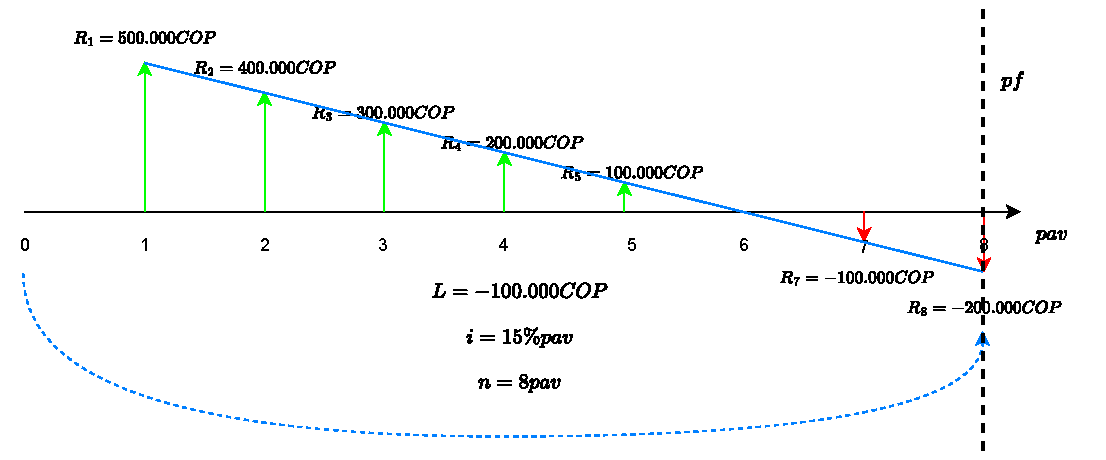
\includegraphics[trim=-5 -5 -5 -5 , scale=0.4]{6_Capitulo/ejemplos/4/Capitulo6Ejemplo4.pdf} }
			
			\\ \hline
			%%%%%%%%%%%%% FIN INSERCIÓN DE IMAGEN
			%%%%%FIN FLUJO DE CAJA
			
			%%%%% INICIO DECLARACIÓN FORMULAS
			%%%%%%%%%%% INICIO TITULO
			\rowcolor[HTML]{FFB183}
			\multicolumn{3}{|c|}{\cellcolor[HTML]{FFB183}\textbf{4. Declaración de fórmulas}}    \\ \hline
			%%%%%%%%%%% FIN TITULO
			%%%%%%%%%%% INICIO MATEMÁTICAS
			
			\multicolumn{3}{|c|}{$VF=R(\frac{(1+i)^{n}-1}{i})+\frac{L}{i}[\frac{(1+i)^{n}-1}{i}-n] \hspace{0.4 cm} \textit{Valor final de gradiente aritmético}$} \\ \hline
			
			%%%%%%%%%% FIN MATEMÁTICAS
			%%%%%% INICIO DESARROLLO MATEMÁTICO
			\rowcolor[HTML]{FFB183}
			%%%%%%%%%%INICIO TITULO
			\multicolumn{3}{|c|}{\cellcolor[HTML]{FFB183}\textbf{5. Desarrollo matemático}}       \\ \hline
			%%%%%%%%%% FIN TITULO
			%%%%%%%%%% INICIO MATEMÁTICAS
			\multicolumn{3}{|c|}{$VF=  500{.}000COP(\frac{(1+0.15)^{8}-1}{0.15})+\frac{-  100{.}000COP}{0.15}[\frac{(1+0.15)^{8}-1}{0.15}-8]\hspace{0.4 cm}\textit{Ecuación de equivalencia}$} \\
			\multicolumn{3}{|c|}{$VF=  3{.}045{.}000 \textit{  COP }$} \\ \hline
			
			
			%%%%%%%%%% FIN MATEMÁTICAS
			%%%%%% FIN DESARROLLO MATEMÁTICO
			%%%%%% INICIO RESPUESTA
			\rowcolor[HTML]{FFB183}
			%%%%%%%%%%INICIO TITULO
			\multicolumn{3}{|c|}{\cellcolor[HTML]{FFB183}\textbf{6. Respuesta}}   \\ \hline
			%%%%%%%%%% FIN TITULO
			%%%%%%%%%% INICIO RESPUESTA MATEMÁTICA
			\multicolumn{3}{|c|}{{$\textit{El monto o valor final del flujo de caja es  3{.}045.000  COP }$}}
			\\ \hline
			%%%%%%%%%% FIN MATEMÁTICAS
			%%%%%% FIN RESPUESTA
		\end{longtable}
		%Se crean dos lineas en blanco para que no quede el siguiente texto tan pegado
		%\newline \newline %USARLO SI CREES QUE ES NECESARIO
	\end{center}
	%%%%%%%%%%%%%%%%%%%%%%%%%%FIN EJERCICIO 4 %%%%%%%%%%%%%%%%%%%%%%%%%%%


\section{Relación entre una tasa de interés anticipada(i$_{a}$) y una tasa vencida(i)}
Para $n = 1$, se tiene
$i = \frac{I}{P}$ \\
Si $I = F  d \land P = F (1 -d)$ \hspace{35 pt}\textit{Tasa nominal anual}\\\\
Remplazando en i: \\
$i = \frac {F d} {F (1-d)}$\\\\
Factorizando F,  se obtiene: \\
$i = \frac{d}{(1 - d)}$\\
Remplazando $d = i_{a} $, se obtiene: \\
$i = \frac{ia}{(1 - ia)}$\\\\
Despejando $i_{a}$: \\
$i_{a} = \frac{i}{(1+i)}$ \\\\
$i = \frac{I}{P} = \frac{F d}{F(1-d)}$\\\\
$i = \frac{d}{1-d}$\\

Reemplazando d = $i_{a}$, se obtiene:\\

$i_{a} = \frac{i}{1+i}$\hspace{35 pt}\textit{Tasa periódica anticipada}\\
$j_{a} = i_{a}  (m)$\hspace{23 pt}\textit{Tasa nominal anual anticipada}\\\\

\section{Tasa de interés nominal anual (j) y tasa efectiva anual (EA)}
Según la Superintendencia Financiera de Colombia, la tasa de interés nominal anual es la tasa que el emisor paga al inversionista por un título valor.
Las tasas nominales anuales corresponden a la anualización de una tasa \textbf{periódica}. \\
De igual forma, pueden tener modalidad vencida o anticipada para la liquidación de intereses.\\

\textbf{Tasa de interés efectiva anual (EA):} La tasa de interés efectiva anual, es el instrumento apropiado para medir y comparar, el rendimiento de distintas alternativas de inversión según la Superintendencia Financiera.\\
Según el profesor Javier Serrano, en el libro “Matemáticas financieras y evaluación de proyectos”, la tasa de interés efectiva anual (EA) corresponde a aquella tasa que paga de una sola vez al final del año.\\

Para calcular la tasa efectiva anual, se parte de la fórmula de equivalencia de tasas en donde el
período es anual vencido.

$(1 + i_1)^{m_1} = (1 + i_2)^{m_2}$ , en donde $i_1$ = tasa periódica, que anualizada ($j_1$) es equivalente a la tasa efectiva anual, para un $m_1 = 1 pav$.\\

IMPORTANTE: La tasa Efectiva Anual es equivalente a la tasa Nominal Anual Año Vencido. (naav) \\


\section{Gráfica de equivalencia de tasas}
Gráfica idónea para realizar una equivalencia entre tasas, utilizando las ecuaciones previamente analizadas, se verá que podemos partir de una tasa cualquiera e ir a otra sin necesidad de información adicional.\\
Los puntos que se han colocado del 1 al 8 solo sirven de identificación.\\
\begin{center}
   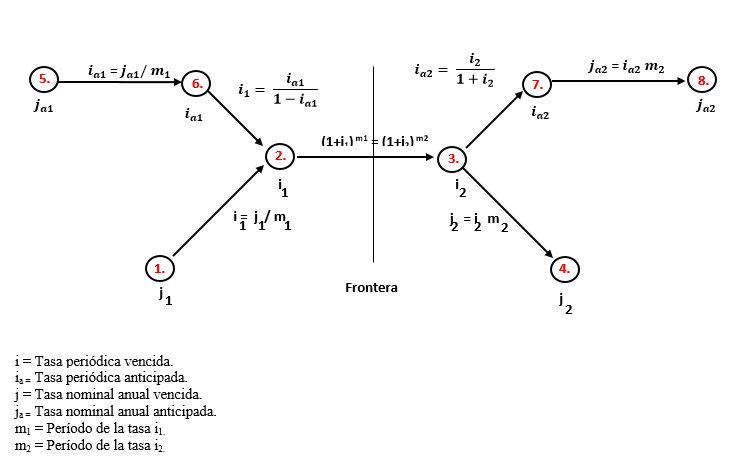
\includegraphics[height = 9.0 cm]{general.png}\\
\end{center}

\textbf{Observación:} Para el uso de la gráfica de equivalencia de tasas, siempre se debe comenzar de un punto de la izquierda y seguir la trayectoria hasta llegar a otro punto situado en la parte derecha.\\
\newpage

\textbf{Ejemplo 5}\\
Hallar el monto, el valor futuro y el valor presente de 20 pagos de 200.000 COP cada uno, suponga una tasa del 24\% nominal anual año vencido.\\ \\
%\newpage %USAR SOLO SI EL SOLUCIÓN QUEDA SOLO Y ES NECESARIO BAJARLO A LA SIGUIENTE PAGINA
\textbf{Solución.}
%La tabla ira centrada
\begin{center}
 \renewcommand{\arraystretch}{1.5}% Margenes de las celdas
 %Creación de la cuadricula de 3 columnas
 \begin{longtable}[H]{|p{0.333\linewidth}|p{0.3333\linewidth}|p{0.3333\linewidth}|}
  \hline
  \multicolumn{3}{|c|}{\cellcolor[HTML]{FFB183}\textbf{1. Declaración de variables}}                   \\ \hline
  $R= 200.000 COP$         & $i=24\% \hspace{1mm} pav$ & $VP = ? COP$                                  \\
  $n=20 \hspace{1mm} pav$ &                            & $VF= ? COP$                                   \\ \hline
  \multicolumn{3}{|c|}{\cellcolor[HTML]{FFB183}\textbf{2. Tabla de flujo de caja}}                     \\ \hline
  \multicolumn{3}{|p{\columnwidth}|}{
  \begin{center}
   \begin{tabular}{ |p{3.5cm}| p{3cm}|}
    \hline

    \textbf{Periodo (psv) } & \textbf{Flujo} \\ \hline
    0                       & -              \\\hline
    1                       &  200.000 COP     \\ \hline
    2                       &  200.000 COP     \\ \hline
    3                       &  200.000 COP     \\ \hline
    4                       &  200.000 COP     \\ \hline
    5                       &  200.000 COP     \\ \hline
    6                       &  200.000 COP     \\ \hline
    7                       &  200.000 COP     \\ \hline
    8                       &  200.000 COP     \\ \hline
    9                       &  200.000 COP     \\ \hline
    10                      &  200.000 COP     \\ \hline
    11                      &  200.000 COP     \\ \hline
    12                      &  200.000 COP     \\ \hline
    13                      &  200.000 COP     \\ \hline
    14                      &  200.000 COP     \\ \hline
    15                      &  200.000 COP     \\ \hline
    16                      &  200.000 COP     \\ \hline
    17                      &  200.000 COP     \\ \hline
    18                      &  200.000 COP     \\ \hline
    19                      &  200.000 COP     \\ \hline
    20                      &  200.000 COP     \\ \hline
   \end{tabular}

  \end{center}
  }                                                                                                   \\ \hline
  \multicolumn{3}{|c|}{\cellcolor[HTML]{FFB183}\textbf{3. Fórmulas utilizadas}}                       \\ \hline
  \multicolumn{3}{|p{\columnwidth}|}{Mediante el uso de Excel:
  \begin{itemize}
   \item VA (Valor actual): Devuelve el valor presente para una inversión
   \item VF (Valor Futuro): Devuelve el valor futuro de una inversión basado en pagos
         periódicos y constantes, y una tasa de interés constante
  \end{itemize}
  }                                                                                                   \\ \hline
  \multicolumn{3}{|c|}{\cellcolor[HTML]{FFB183}\textbf{4. Desarrollo en Excel}}                       \\ \hline
  \multicolumn{3}{|l|}{Se aplicarán las funciones VA y VF de la siguiente forma:}                     \\
  \multicolumn{3}{|c|}{ 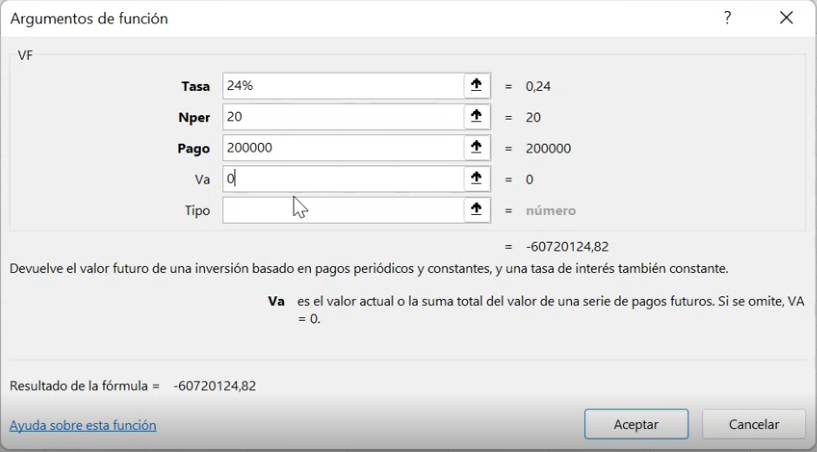
\includegraphics[trim=-5 -5 -5 -5 ,width=1\columnwidth]{5/Ejem5.1.PNG}}        \\
  \multicolumn{3}{|l|}{=VF(0,24;20;-200000;0) con referencia en la hoja de Excel usada para el ejercicio.}    \\
  \multicolumn{3}{|c|}{ 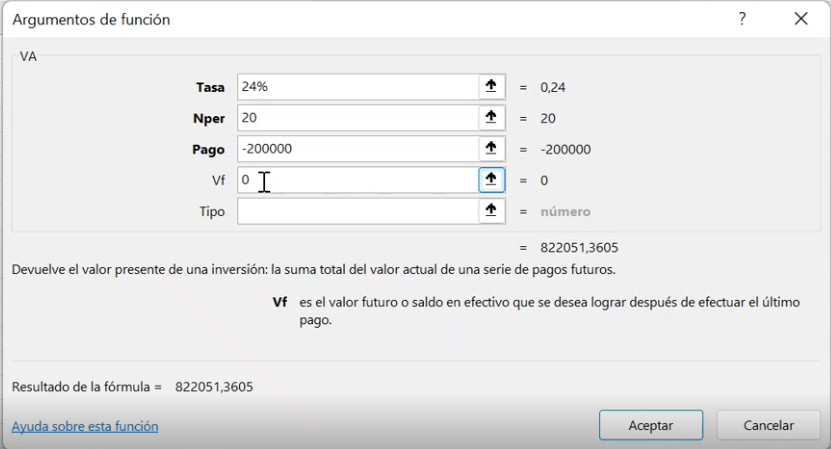
\includegraphics[trim=-5 -5 -5 -5 ,width=1\columnwidth]{5/Ejem5.2.PNG}}        \\
  \multicolumn{3}{|l|}{=VA(0,24;20;-200000;0) con referencia en la hoja de Excel usada para el ejercicio.} \\ \hline
  \multicolumn{3}{|c|}{\cellcolor[HTML]{FFB183}\textbf{5. Respuesta}}                                 \\ \hline
  \multicolumn{3}{|p{\columnwidth}|}{
  El valor presente (VP) o valor actual (VA) es 822.051 COP y el valor futuro (VF) es 60.720.114 COP 
  }                                                                                                   \\ \hline
  \multicolumn{3}{|c|}{\cellcolor[HTML]{FFB183}\textbf{6. Gráfica}}                                   \\ \hline
  \multicolumn{3}{|c|}{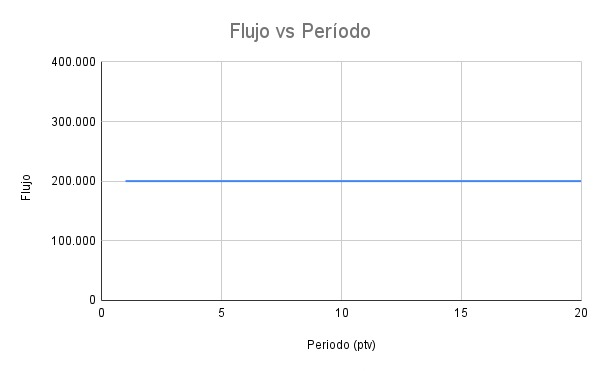
\includegraphics[trim=-5 -5 -5 -5 ,width=0.7\columnwidth]{4/flujovsperiodo.png}}      \\ \hline
 \end{longtable}
 %\newline \newline %USARLO SI CREES QUE ES NECESARIO
\end{center}

	
	\textbf{Ejemplo 6}\\
	Calcular el valor presente de una serie infinita de egresos que crecen en  10{.}000COP, si el primer egreso es de  200{.}000COP y la tasa es del 3\% periódica mes vencido.\\
	
	\newpage
	
	%%%%%%%%%%%%%%%%%%% EJERCICIO 6 %%%%%%
	
	%\newpage %USAR SOLO SI EL SOLUCIÓN QUEDA SOLO Y ES NECESARIO BAJARLO A LA SIGUIENTE PAGINA
	\textbf{Solución.}\\
	%La tabla ira centrada
	\begin{center}
		\renewcommand{\arraystretch}{1.6}% Margenes de las celdas
		%Creación de la cuadricula de 3 columnas
		\begin{longtable}[H]{|c|c|c|}
			%Creamos una linea horizontal
			\hline
			%Definimos el color de la primera fila
			\rowcolor[HTML]{FFB183}
			%%%%% INICIO ASIGNACIÓN FECHA FOCAL %%%%%%%
			%%%%%%%%%% INICIO TITULO
			%Lo que se hace aquí es mezclar las 3 columnas en una sola
			\multicolumn{3}{|c|}{\cellcolor[HTML]{FFB183}\textbf{1. Asignación período focal}}  \\ \hline
			\multicolumn{3}{|c|}{$pf = \textit{0 pmv}$}   \\\hline
			%%%%%%%%%% FIN TITULO
			%%%%% INICIO DECLARACIÓN DE VARIABLES %%%%%%%
			%%%%%%%%%% INICIO TITULO
			%Lo que se hace aquí es mezclar las 3 columnas en una sola
			\multicolumn{3}{|c|}{\cellcolor[HTML]{FFB183}\textbf{2. Declaración de variables}}   \\ \hline
			%%%%%%%%%% FIN TITULO
			%%%%%%%%%% INICIO DE MATEMÁTICAS
			%Cada & hace referencia al paso de la siguiente columna
			\multicolumn{2}{|c|}{\textbf{$\hspace{3.5 cm}\textit{}\hspace{3.5 cm}$}} & \textbf{$\hspace{3.5 cm}\textit{}\hspace{3.5 cm}$} \\ 
			\multicolumn{2}{|c|}{$\hspace{2 cm}L=  10{.}000COP \hspace{2 cm}$} & {$i=3\% \textit{ pmv}$} \\
			\multicolumn{2}{|c|}{$\hspace{2 cm}R=   200{.}000COP \hspace{2 cm}$} & $n=\infty \textit{ pmv}$ \\ 	
			\multicolumn{2}{|c|}{$\hspace{2cm} VP = ? COP \hspace{2 cm}$ } & $$\\ \hline
			%%%%%%%%%% FIN DE MATEMÁTICAS
			%%%%% FIN DECLARACIÓN DE VARIABLES
			
			%%%%% INICIO FLUJO DE CAJA
			\rowcolor[HTML]{FFB183}
			\multicolumn{3}{|c|}{\cellcolor[HTML]{FFB183}\textbf{3. Diagrama de flujo de caja}} \\ \hline
			%Mezclamos 3 columnas y pondremos el dibujo
			%%%%%%%%%%%%% INSERCIÓN DE LA IMAGEN
			%Deberán descargar las imágenes respectivas del drive y pegarlas en la carpeta
			%n_capitulo/img/ejemplos/1/capitulo1ejemplo1.pdf  (el /1/ es el numero del ejemplo)
			\multicolumn{3}{|c|}{ \includegraphics[trim=-5 -5 -5 -5 , scale=0.6]{6_Capitulo/img/ejemplos/6/capitulo6ejemplo6.pdf} }
			
			\\ \hline
			%%%%%%%%%%%%% FIN INSERCIÓN DE IMAGEN
			%%%%%FIN FLUJO DE CAJA
			
			%%%%% INICIO DECLARACIÓN FORMULAS
			%%%%%%%%%%% INICIO TITULO
			\rowcolor[HTML]{FFB183}
			\multicolumn{3}{|c|}{\cellcolor[HTML]{FFB183}\textbf{4. Declaración de fórmulas}}    \\ \hline
			%%%%%%%%%%% FIN TITULO
			%%%%%%%%%%% INICIO MATEMÁTICAS
			
			\multicolumn{3}{|c|}{$VP=(\frac{R}{i})+(\frac{L}{i^2}) \hspace{0.4 cm} \textit{Valor presente de un gradiente aritmetico}$} \\ \hline
			
			%%%%%%%%%% FIN MATEMÁTICAS
			%%%%%% INICIO DESARROLLO MATEMÁTICO
			\rowcolor[HTML]{FFB183}
			%%%%%%%%%%INICIO TITULO
			\multicolumn{3}{|c|}{\cellcolor[HTML]{FFB183}\textbf{5. Desarrollo matemático}}       \\ \hline
			%%%%%%%%%% FIN TITULO
			%%%%%%%%%% INICIO MATEMÁTICAS
			\multicolumn{3}{|c|}{$VP=(\frac{ 200{.}000}{0,03})+(\frac{  10{.}000COP}{0,03^2}) \hspace{0.2 cm}\rightarrow \hspace{0.2 cm}VP= COP 17{.}777{.}778$} \\ \hline
			
			%%%%%%%%%% FIN MATEMÁTICAS
			%%%%%% FIN DESARROLLO MATEMÁTICO
			%%%%%% INICIO RESPUESTA
			\rowcolor[HTML]{FFB183}
			%%%%%%%%%%INICIO TITULO
			\multicolumn{3}{|c|}{\cellcolor[HTML]{FFB183}\textbf{6. Respuesta}}   \\ \hline
			%%%%%%%%%% FIN TITULO
			%%%%%%%%%% INICIO RESPUESTA MATEMÁTICA
			\multicolumn{3}{|c|}{$ VP=  17{.}777.78 COP$} 
			\\ \hline
			%%%%%%%%%% FIN MATEMÁTICAS
			%%%%%% FIN RESPUESTA
		\end{longtable}
		%Se crean dos lineas en blanco para que no quede el siguiente texto tan pegado
		%\newline \newline %USARLO SI CREES QUE ES NECESARIO
	\end{center}
	%%%%%%%%%%%%%%%%%%%%%%%%%%FIN EJERCICIO 6 %%%%%%%%%%%%%%%%%%%%%%%%%%%

\textbf{Ejemplo 7:}\\
Hallar el valor presente de 10 egresos anuales, si el primer egreso es de  500.000 COP y cada egreso subsiguiente crece un 20\% pav. Suponga una tasa del 20\% periódica anual vencida.\\

	%%%%%%%%%%%%%%%%%%% EJERCICIO 7 %%%%%%

%\newpage %USAR SOLO SI EL SOLUCIÓN QUEDA SOLO Y ES NECESARIO BAJARLO A LA SIGUIENTE PAGINA
\textbf{Solución.}\\
%La tabla ira centrada
\begin{center}
	\renewcommand{\arraystretch}{1.6}% Margenes de las celdas
	%Creación de la cuadricula de 3 columnas
	\begin{longtable}[H]{|c|c|c|}
		%Creamos una linea horizontal
		\hline
		%Definimos el color de la primera fila
		\rowcolor[HTML]{FFB183}
		%%%%% INICIO ASIGNACIÓN FECHA FOCAL %%%%%%%
		%%%%%%%%%% INICIO TITULO
		%Lo que se hace aquí es mezclar las 3 columnas en una sola
		\multicolumn{3}{|c|}{\cellcolor[HTML]{FFB183}\textbf{1. Asignación período focal}}  \\ \hline
		\multicolumn{3}{|c|}{$pf = \textit{0 pav}$}   \\\hline
		%%%%%%%%%% FIN TITULO
		%%%%% INICIO DECLARACIÓN DE VARIABLES %%%%%%%
		%%%%%%%%%% INICIO TITULO
		%Lo que se hace aquí es mezclar las 3 columnas en una sola
		\multicolumn{3}{|c|}{\cellcolor[HTML]{FFB183}\textbf{2. Declaración de variables}}   \\ \hline
		%%%%%%%%%% FIN TITULO
		%%%%%%%%%% INICIO DE MATEMÁTICAS
		%Cada & hace referencia al paso de la siguiente columna
		\multicolumn{2}{|c|}{\textbf{$\hspace{3.5 cm}\textit{}\hspace{3.5 cm}$}} & \textbf{$\hspace{3.5 cm}\textit{}\hspace{3.5 cm}$} \\ 
		\multicolumn{2}{|c|}{$\hspace{2 cm}R=  500{.}000 COP \hspace{2 cm}$} & $i=20\% \textit{ pav}$ \\
		\multicolumn{2}{|c|}{$\hspace{2 cm}g=20\% \hspace{2 cm}$} & $n=\textit{10 pav}$ \\
		\multicolumn{2}{|c|}{$\hspace{2 cm}VP=   ?COP \hspace{2 cm}$} & \\ \hline	
		
		
		%%%%%%%%%% FIN DE MATEMÁTICAS
		%%%%% FIN DECLARACIÓN DE VARIABLES
		
		%%%%% INICIO FLUJO DE CAJA
		\rowcolor[HTML]{FFB183}
		\multicolumn{3}{|c|}{\cellcolor[HTML]{FFB183}\textbf{3. Diagrama de flujo de caja}} \\ \hline
		%Mezclamos 3 columnas y pondremos el dibujo
		%%%%%%%%%%%%% INSERCIÓN DE LA IMAGEN
		%Deberán descargar las imágenes respectivas del drive y pegarlas en la carpeta
		%n_capitulo/img/ejemplos/1/capitulo1ejemplo1.pdf  (el /1/ es el numero del ejemplo)
		\multicolumn{3}{|c|}{ 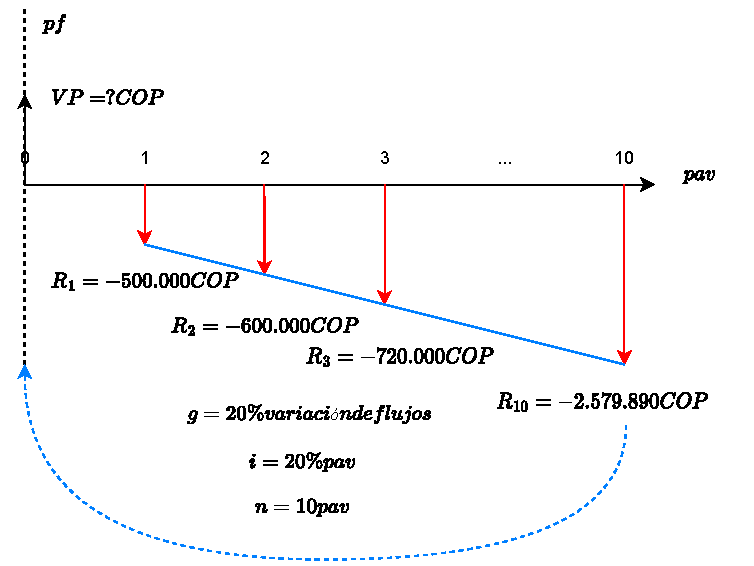
\includegraphics[trim=-5 -5 -5 -5 , scale=0.5]{6_Capitulo/img/ejemplos/7/Capitulo6Ejemplo7.pdf} }
		
		\\ \hline
		%%%%%%%%%%%%% FIN INSERCIÓN DE IMAGEN
		%%%%%FIN FLUJO DE CAJA
		
		%%%%% INICIO DECLARACIÓN FORMULAS
		%%%%%%%%%%% INICIO TITULO
		\rowcolor[HTML]{FFB183}
		\multicolumn{3}{|c|}{\cellcolor[HTML]{FFB183}\textbf{4. Declaración de fórmulas}}    \\ \hline
		%%%%%%%%%%% FIN TITULO
		%%%%%%%%%%% INICIO MATEMÁTICAS
		
		\multicolumn{3}{|c|}{$VP=(\frac{(R)(n)}{1+i}) \hspace{0.4 cm} \textit{Valor presente de un gradiente geometrico para i=g}$} \\ 
		\multicolumn{3}{|c|}{$R_n=(R_1(1+g)^{n-1}) \hspace{0.4 cm} \textit{Valor del flujo de un gradiente geométrico}$} \\ \hline
		
		%%%%%%%%%% FIN MATEMÁTICAS
		%%%%%% INICIO DESARROLLO MATEMÁTICO
		\rowcolor[HTML]{FFB183}
		%%%%%%%%%%INICIO TITULO
		\multicolumn{3}{|c|}{\cellcolor[HTML]{FFB183}\textbf{5. Desarrollo matemático}}       \\ \hline
		%%%%%%%%%% FIN TITULO
		%%%%%%%%%% INICIO MATEMÁTICAS
		
		\multicolumn{3}{|c|}{$VP=(\frac{( 500{.}000COP)(10)}{1+0,2}) \hspace{0.2 cm}\rightarrow \hspace{0.2 cm} VP=  4{.}166{.}667COP$} \\ \hline
		%%%%%%%%%% FIN MATEMÁTICAS
		%%%%%% FIN DESARROLLO MATEMÁTICO
		%%%%%% INICIO RESPUESTA
		\rowcolor[HTML]{FFB183}
		%%%%%%%%%%INICIO TITULO
		\multicolumn{3}{|c|}{\cellcolor[HTML]{FFB183}\textbf{6. Respuesta}}   \\ \hline
		%%%%%%%%%% FIN TITULO
		%%%%%%%%%% INICIO RESPUESTA MATEMÁTICA
		\multicolumn{3}{|c|}{${VP=  4{.}166{.}667 COP}$} 
		\\ \hline
		%%%%%%%%%% FIN MATEMÁTICAS
		%%%%%% FIN RESPUESTA
	\end{longtable}
	%Se crean dos lineas en blanco para que no quede el siguiente texto tan pegado
	%\newline \newline %USARLO SI CREES QUE ES NECESARIO
\end{center}
%%%%%%%%%%%%%%%%%%%%%%%%%%FIN EJERCICIO 7 %%%%%%%%%%%%%%%%%%%%%%%%%%%

\newpage
\textbf{Ejemplo 8}\\
Supongamos que un inversionista desea adquirir la aceptación bancaria del ejemplo anterior, la cual figura con una tasa de registro del 30\% periódico 40 días vencido y con precio de registro $P_r =  97,65 COP$ pero él también sabe que para adquirirla deberá pagar una comisión a un corredor de bolsa lo cual hará variar el precio que él debe pagar y también la rentabilidad que él pueda obtener. Supongamos que la comisión que cobra un corredor por la compra es del 0,475\% periodo 40 días periodo vencido ¿Cuál es el precio del inversionista Pc =  ? COP , que incluye la comisión del comisionista vendedor, el precio de registro y la comisión de bolsa del comprador. El punto de referencia es el precio de registro $P_r$ ¿Cuál es la rentabilidad del inversionista $i_c =? \%?$ periódica 40 días vencido, o $j=? \hspace{0.5mm} nadv$
%\newpage %USAR SOLO SI EL SOLUCIÓN QUEDA SOLO Y ES NECESARIO BAJARLO A LA SIGUIENTE PAGINA

\textbf{Solución.}
%La tabla ira centrada
\begin{center}
 \renewcommand{\arraystretch}{1.5}% Margenes de las celdas
 %Creación de la cuadricula de 3 columnas
 \begin{longtable}[H]{|p{0.5\linewidth}|p{0.5\linewidth}|}
  %Creamos una linea horizontal
  \hline
  %Definimos el color de la primera fila
  \rowcolor[HTML]{FFB183}
  %%%%% INICIO ASIGNACIÓN FECHA FOCAL %%%%%%%
  %%%%%%%%%% INICIO TITULO
  %Lo que se hace aquí es mezclar las 3 columnas en una sola
  \multicolumn{2}{|c|}{\cellcolor[HTML]{FFB183}\textbf{1. Asignación período focal}}                  \\ \hline
  %%%%%%%%%% FIN TITULO
  %%%%% INICIO DECLARACIÓN DE VARIABLES %%%%%%%
  \multicolumn{2}{|c|}{$pf = 40 \textit{ pdv}$}                                                     \\ \hline
  %%%%%%%%%% INICIO TITULO
  %Lo que se hace aquí es mezclar las 3 columnas en una sola
  \multicolumn{2}{|c|}{\cellcolor[HTML]{FFB183}\textbf{2. Declaración de variables}}                \\ \hline
  %%%%%%%%%% FIN TITULO
  %%%%%%%%%% INICIO DE MATEMÁTICAS
  %Cada & hace referencia al paso de la siguiente columna
  $i_c = 30\% -0,475\% = 29,525\% \hspace{1mm} p40dv$ & $P_R=?$                                     \\
  $P_c =  ? COP$                                         &                                             \\
  $n= \frac{40}{365} \hspace{1mm} p(40das) $          &                                             \\ \hline
  %%%%%%%%%% FIN DE MATEMÁTICAS
  %%%%% FIN DECLARACIÓN DE VARIABLES

  \rowcolor[HTML]{FFB183}
  \multicolumn{2}{|c|}{\cellcolor[HTML]{FFB183}\textbf{3. Diagrama de flujo de caja}}               \\ \hline
  \multicolumn{2}{|c|}{ 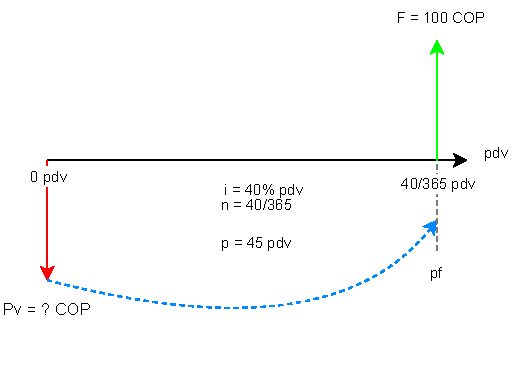
\includegraphics[trim=-78 0 -78 0]{3_Capitulo/img/ejemplos/8/capitulo3ejercicio8.pdf} }  \\ \hline
  %%%%% INICIO FLUJO DE CAJA
  \rowcolor[HTML]{FFB183}
  \multicolumn{2}{|c|}{\cellcolor[HTML]{FFB183}\textbf{4. DECLARACIÓN de formulas}}                 \\ \hline
  %Mezclamos 3 columnas y pondremos el dibujo
  %%%%%%%%%%%%% INSERCIÓN DE LA IMAGEN
  %Deberán descargar las imágenes respectivas del drive y pegarlas en la carpeta
  %n_capitulo/img/ejemplos/1/capitulo1ejemplo1.pdf  (el /1/ es el numero del ejemplo)
  \multicolumn{2}{|c|}{ $P = F(1 + i)^n $ Valor presente }                                          \\ \hline
  %%%%%%%%%%%%% FIN INSERCIÓN DE IMAGEN
  %%%%%FIN FLUJO DE CAJA


  %%%%%% INICIO DESARROLLO MATEMÁTICO
  \rowcolor[HTML]{FFB183}
  %%%%%%%%%%INICIO TITULO
  \multicolumn{2}{|c|}{\cellcolor[HTML]{FFB183}\textbf{5. Desarrollo matemático}}                   \\ \hline
  %%%%%%%%%% FIN TITULO
  %%%%%%%%%% INICIO MATEMÁTICAS
  \multicolumn{2}{|C{\linewidth}|}{
  $P_c =  100 COP(1 + 0,29525)\frac{40}{365} = 97,204 COP$ Ecuación de valor

  $P_R = 0,972047( 5{.}000{.}000 COP) =  4{.}860{.}245 COP$

  $P_c - P_R =  4{.}860{.}235 COP -  4{.}858{.}285 COP = 1{.}950 COP$
  }                                                                                                 \\ \hline

  %%%%%%%%%% FIN MATEMÁTICAS
  %%%%%% FIN DESARROLLO MATEMÁTICO
  %%%%%% INICIO RESPUESTA
  \rowcolor[HTML]{FFB183}
  %%%%%%%%%%INICIO TITULO
  \multicolumn{2}{|c|}{\cellcolor[HTML]{FFB183}\textbf{6. Respuesta}}                               \\ \hline
  %%%%%%%%%% FIN TITULO
  %%%%%%%%%% INICIO RESPUESTA MATEMÁTICA
  \multicolumn{2}{|C{\textwidth}|}{
  $P_R =  4{.}860{.}245 COP$
  }                                                                                                 \\ \hline


  %%%%%%%%%% FIN MATEMÁTICAS
  %%%%%% FIN RESPUESTA
 \end{longtable}
 %Se crean dos lineas en blanco para que no quede el siguiente texto tan pegado
 %\newline \newline %USARLO SI CREES QUE ES NECESARIO
\end{center}
\textbf{Ejemplo 9}\\
Elaborar una tabla para amortizar la suma de  100.000 COP en 4 pagos, suponiendo una tasa del 8\% periódica anual vencida:
\begin{itemize}
	\item a. Crecimiento geométrico periódico de 10\% de los flujos
	\item b. Decrecimiento geométrico periódico de 10\% de los flujos
\end{itemize}
	
	%%%%%%%%%%%%%%%%%%% EJERCICIO 9a %%%%%%

%\newpage %USAR SOLO SI EL SOLUCIÓN QUEDA SOLO Y ES NECESARIO BAJARLO A LA SIGUIENTE PAGINA
\textbf{Solución a.}\\
%La tabla ira centrada
\begin{center}
	\renewcommand{\arraystretch}{1.6}% Margenes de las celdas
	%Creación de la cuadricula de 3 columnas
	\begin{longtable}[H]{|c|c|c|}
		%Creamos una linea horizontal
		\hline
		%Definimos el color de la primera fila
		\rowcolor[HTML]{FFB183}
		%%%%% INICIO ASIGNACIÓN FECHA FOCAL %%%%%%%
		%%%%%%%%%% INICIO TITULO
		%Lo que se hace aquí es mezclar las 3 columnas en una sola
		\multicolumn{3}{|c|}{\cellcolor[HTML]{FFB183}\textbf{1. Asignación período focal}}  \\ \hline
		\multicolumn{3}{|c|}{$pf = \textit{0 pav}$}   \\\hline
		%%%%%%%%%% FIN TITULO
		%%%%% INICIO DECLARACIÓN DE VARIABLES %%%%%%%
		%%%%%%%%%% INICIO TITULO
		%Lo que se hace aquí es mezclar las 3 columnas en una sola
		\multicolumn{3}{|c|}{\cellcolor[HTML]{FFB183}\textbf{2. Declaración de variables}}   \\ \hline
		%%%%%%%%%% FIN TITULO
		%%%%%%%%%% INICIO DE MATEMÁTICAS
		%Cada & hace referencia al paso de la siguiente columna
		\multicolumn{2}{|c|}{$\hspace{2 cm}R=  100{.}000 COP \hspace{2 cm}$} & $i=8\% \textit{ pav}$ \\
		\multicolumn{2}{|c|}{$\hspace{2 cm}n=4  \textit{ pav} \hspace{2 cm}$} & $g=10\% \textit{creicente geometrico periódico con } g \neq i$ \\ \hline	
		
		
		%%%%%%%%%% FIN DE MATEMÁTICAS
		%%%%% FIN DECLARACIÓN DE VARIABLES
		
		%%%%% INICIO FLUJO DE CAJA
		\rowcolor[HTML]{FFB183}
		\multicolumn{3}{|c|}{\cellcolor[HTML]{FFB183}\textbf{3. Diagrama de flujo de caja}} \\ \hline
		%Mezclamos 3 columnas y pondremos el dibujo
		%%%%%%%%%%%%% INSERCIÓN DE LA IMAGEN
		%Deberán descargar las imágenes respectivas del drive y pegarlas en la carpeta
		%n_capitulo/img/ejemplos/1/capitulo1ejemplo1.pdf  (el /1/ es el numero del ejemplo)
		\multicolumn{3}{|c|}{ 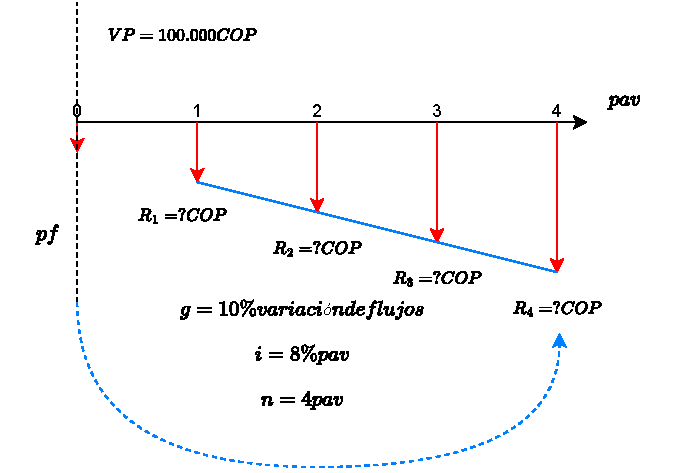
\includegraphics[trim=-5 -5 -5 -5 , scale=0.6]{6_Capitulo/img/ejemplos/9/Capitulo6Ejemplo9a.pdf} }
		\\ \hline
		%%%%%%%%%%%%% FIN INSERCIÓN DE IMAGEN
		%%%%%FIN FLUJO DE CAJA
		
		%%%%% INICIO DECLARACIÓN FORMULAS
		%%%%%%%%%%% INICIO TITULO
		\rowcolor[HTML]{FFB183}
		\multicolumn{3}{|c|}{\cellcolor[HTML]{FFB183}\textbf{4. Declaración de fórmulas}}    \\ \hline
		%%%%%%%%%%% FIN TITULO
		%%%%%%%%%%% INICIO MATEMÁTICAS
		\multicolumn{3}{|c|}{$VP=(\frac{(R)[(1+g)^{n}(1+i)^{-n}-1]}{g-i}) \hspace{0.4 cm} \textit{Valor presente de un gradiente aritmético }$} \\  
		\multicolumn{3}{|c|}{$R_n=(R_1(1+g)^{n-1}) \hspace{0.4 cm} \textit{Valor del flujo de n gradiente geométrico}$} \\ \hline
		
		%%%%%%%%%% FIN MATEMÁTICAS
		%%%%%% INICIO DESARROLLO MATEMÁTICO
		\rowcolor[HTML]{FFB183}
		%%%%%%%%%%INICIO TITULO
		\multicolumn{3}{|c|}{\cellcolor[HTML]{FFB183}\textbf{5. Desarrollo matemático}}       \\ \hline
		%%%%%%%%%% FIN TITULO
		%%%%%%%%%% INICIO MATEMÁTICAS
		\multicolumn{3}{|c|}{$100{.}000COP=(\frac{(R_1)[(1+0.1)^{4}(1+0.08)^{-4}-1]}{0.1-0.08})$} \\
		\multicolumn{3}{|c|}{$R_1=  26{.}261.47 COP$}\\ 
		\multicolumn{3}{|c|}{$R_2=  26{.}261.47(1+0.1) COP=   28{.}887.61COP$}\\
		\multicolumn{3}{|c|}{$R_3=  26{.}261.47(1+0.1)^2 COP=   31{.}776.38COP$}\\
		\multicolumn{3}{|c|}{$R_4=  26{.}261.47(1+0.1)^3 COP=   34{.}954.01COP$}\\ \hline
		%%%%%%%%%% FIN MATEMÁTICAS
		%%%%%% FIN DESARROLLO MATEMÁTICO
		%%%%%% INICIO RESPUESTA
		\rowcolor[HTML]{FFB183}
		%%%%%%%%%%INICIO TITULO
		\multicolumn{3}{|c|}{\cellcolor[HTML]{FFB183}\textbf{6. Respuesta}}   \\ \hline
		%%%%%%%%%% FIN TITULO
		%%%%%%%%%% INICIO RESPUESTA MATEMÁTICA
		\multicolumn{3}{|c|}{$R_1=  26{.}261COP$}\\ 
		\multicolumn{3}{|c|}{$R_2=  28{.}888 COP$}\\
		\multicolumn{3}{|c|}{$R_3=  31{.}776 COP$}\\
		\multicolumn{3}{|c|}{$R_4=  34{.}954 COP$}\\ \hline
		%%%%%%%%%% FIN MATEMÁTICAS
		%%%%%% FIN RESPUESTA
	\end{longtable}
	%Se crean dos lineas en blanco para que no quede el siguiente texto tan pegado
	%\newline \newline %USARLO SI CREES QUE ES NECESARIO
\end{center}

%%%%%%%%%%%%%%%%%%%%%%%%%%FIN EJERCICIO 9a %%%%%%%%%%%%%%%%%%%%%%%%%%%
	      \begin{spacing}{1.1}
	      	\begin{center}
	      		\begin{tabular}{|p{1cm}|p{2cm}|p{2.1cm}|p{2cm}|p{3cm}|}
	      			\hline
	      			\rowcolor{white!50}
	      			\textbf{n\ } & \textbf{Saldo Deuda COP} & \textbf{Intereses  COP} & \textbf{Pago COP} & \textbf{Amortización COP } \\ \hline
	      			
	      			0            &   100.000         &      -       &   -    &        -      \\ \hline
	      			1            &   81.739             &   8.000           &   26.261       &   18.261            \\ \hline
	      			2            &   59.390             &   6539,13              &   28.888       &   22.348,88              \\ \hline
	      			3            &   32.365.21            &   4751,2             &   31.776      &   27.024,79              \\ \hline
	      			4            &   0            &   2589,22            &   34.954       &   32.365,21              \\ \hline
	      		\end{tabular}
	      	\end{center}
	      \end{spacing}

	%%%%%%%%%%%%%%%%%%% EJERCICIO 9b %%%%%%

%\newpage %USAR SOLO SI EL SOLUCIÓN QUEDA SOLO Y ES NECESARIO BAJARLO A LA SIGUIENTE PAGINA
\textbf{Solución b.}\\
%La tabla ira centrada
\begin{center}
	\renewcommand{\arraystretch}{1.6}% Margenes de las celdas
	%Creación de la cuadricula de 3 columnas
	\begin{longtable}[H]{|c|c|c|}
		%Creamos una linea horizontal
		\hline
		%Definimos el color de la primera fila
		\rowcolor[HTML]{FFB183}
		%%%%% INICIO ASIGNACIÓN FECHA FOCAL %%%%%%%
		%%%%%%%%%% INICIO TITULO
		%Lo que se hace aquí es mezclar las 3 columnas en una sola
		\multicolumn{3}{|c|}{\cellcolor[HTML]{FFB183}\textbf{1. Asignación período focal}}  \\ \hline
		\multicolumn{3}{|c|}{$pf = \textit{0 pav}$}   \\\hline
		%%%%%%%%%% FIN TITULO
		%%%%% INICIO DECLARACIÓN DE VARIABLES %%%%%%%
		%%%%%%%%%% INICIO TITULO
		%Lo que se hace aquí es mezclar las 3 columnas en una sola
		\multicolumn{3}{|c|}{\cellcolor[HTML]{FFB183}\textbf{2. Declaración de variables}}   \\ \hline
		%%%%%%%%%% FIN TITULO
		%%%%%%%%%% INICIO DE MATEMÁTICAS
		%Cada & hace referencia al paso de la siguiente columna
		\multicolumn{2}{|c|}{$\hspace{2 cm}VP= 100{.}000 COP \hspace{2 cm}$} & $i=8\% \textit{ pav}$ \\
		\multicolumn{2}{|c|}{$\hspace{2 cm}n=4  \textit{ pav} \hspace{2 cm}$} & $g=-10\% \textit{decreicente con } g \neq i$ \\ \hline	
		
		%%%%%%%%%% FIN DE MATEMÁTICAS
		%%%%% FIN DECLARACIÓN DE VARIABLES
		
		%%%%% INICIO FLUJO DE CAJA
		\rowcolor[HTML]{FFB183}
		\multicolumn{3}{|c|}{\cellcolor[HTML]{FFB183}\textbf{3. Diagrama de flujo de caja}} \\ \hline
		%Mezclamos 3 columnas y pondremos el dibujo
		%%%%%%%%%%%%% INSERCIÓN DE LA IMAGEN
		%Deberán descargar las imágenes respectivas del drive y pegarlas en la carpeta
		%n_capitulo/img/ejemplos/1/capitulo1ejemplo1.pdf  (el /1/ es el numero del ejemplo)
		\multicolumn{3}{|c|}{ 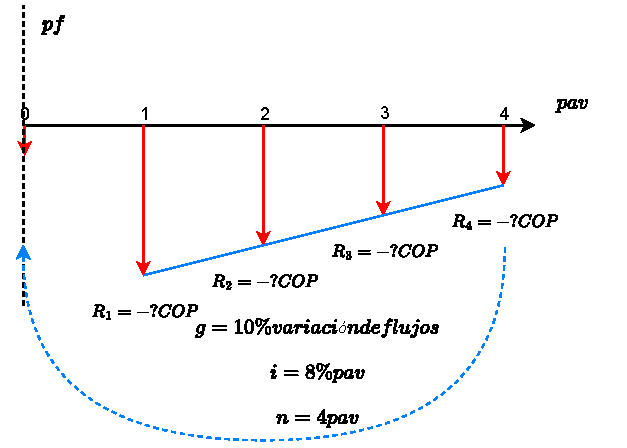
\includegraphics[trim=-5 -5 -5 -5 , scale=0.6]{6_Capitulo/img/ejemplos/9/Capitulo6Ejemplo9b.pdf} }
		\\ \hline
		%%%%%%%%%%%%% FIN INSERCIÓN DE IMAGEN
		%%%%%FIN FLUJO DE CAJA
		
		%%%%% INICIO DECLARACIÓN FORMULAS
		%%%%%%%%%%% INICIO TITULO
		\rowcolor[HTML]{FFB183}
		\multicolumn{3}{|c|}{\cellcolor[HTML]{FFB183}\textbf{4. Declaración de fórmulas}}    \\ \hline
		%%%%%%%%%%% FIN TITULO
		%%%%%%%%%%% INICIO MATEMÁTICAS
		\multicolumn{3}{|c|}{$VP=(\frac{(R)[(1+g)^{n}(1+i)^{-n}-1]}{g-i}) \hspace{0.4 cm} \textit{Valor presente de un gradiente aritmético }$} \\  
		\multicolumn{3}{|c|}{$R_n=(R_1(1+g)^{n-1}) \hspace{0.4 cm} \textit{Valor del flujo de n gradiente geométrico}$} \\ \hline
		
		%%%%%%%%%% FIN MATEMÁTICAS
		%%%%%% INICIO DESARROLLO MATEMÁTICO
		\rowcolor[HTML]{FFB183}
		%%%%%%%%%%INICIO TITULO
		\multicolumn{3}{|c|}{\cellcolor[HTML]{FFB183}\textbf{5. Desarrollo matemático}}       \\ \hline
		%%%%%%%%%% FIN TITULO
		%%%%%%%%%% INICIO MATEMÁTICAS
		\multicolumn{3}{|c|}{$  100{.}000COP=(\frac{(R_1)[(1-0.1)^{4}(1+0.08)^{-4}-1]}{-0.1-0.08})$} \\
		\multicolumn{3}{|c|}{$R_1=  34{.}766 COP$}\\ 
		\multicolumn{3}{|c|}{$R_2=  34{.}766.02COP(1-0.1)  =   31{.}289.42COP$}\\
		\multicolumn{3}{|c|}{$R_3=  34{.}766.02COP(1-0.1)^2 =   28{.}160.48COP$}\\
		\multicolumn{3}{|c|}{$R_4=  34{.}766.02COP(1-0.1)^3 =   25{.}344.43COP$}\\ \hline
		%%%%%%%%%% FIN MATEMÁTICAS
		%%%%%% FIN DESARROLLO MATEMÁTICO
		%%%%%% INICIO RESPUESTA
		\rowcolor[HTML]{FFB183}
		%%%%%%%%%%INICIO TITULO
		\multicolumn{3}{|c|}{\cellcolor[HTML]{FFB183}\textbf{6. Respuesta}}   \\ \hline
		%%%%%%%%%% FIN TITULO
		%%%%%%%%%% INICIO RESPUESTA MATEMÁTICA
		\multicolumn{3}{|c|}{$R_1=  34{.}766COP$}\\ 
		\multicolumn{3}{|c|}{$R_2=  31{.}289COP$}\\
		\multicolumn{3}{|c|}{$R_3=  28{.}160COP$}\\
		\multicolumn{3}{|c|}{$R_4=  25{.}344COP$}\\ \hline
		%%%%%%%%%% FIN MATEMÁTICAS
		%%%%%% FIN RESPUESTA
	\end{longtable}
	%Se crean dos lineas en blanco para que no quede el siguiente texto tan pegado
	%\newline \newline %USARLO SI CREES QUE ES NECESARIO
\end{center}

%%%%%%%%%%%%%%%%%%%%%%%%%%FIN EJERCICIO 9b %%%%%%%%%%%%%%%%%%%%%%%%%%%
	      
	      \begin{spacing}{1.1}
		      \begin{center}
			      \begin{tabular}{|p{1cm}|p{2cm}|p{2.1cm}|p{2cm}|p{2.5cm}|}
				      \hline
				      \rowcolor{white!50}
				      \textbf{n\ } & \textbf{Saldo Deuda COP} & \textbf{Intereses COP } & \textbf{Pago COP } & \textbf{Amortización COP} \\ \hline
				      
				      0            &   100.000         & -    & -  & -    \\ \hline
				      1            &   73.234           &   8.000          &   34.766      &   26.766             \\ \hline
				      2            &   47.803,72           &   5858,72             &   31.289      &   25.430,28             \\ \hline
				      3            &   23.468,01           &   3824,29             &   28.160      &   24.335,7            \\ \hline
				      4            &   0               &   1877,44             &   25.344,73      &   23.468,01             \\ \hline
			      \end{tabular}
		      \end{center}
	      \end{spacing}

%%%%%%%%%%%%%%%%%%%%%%%%%%EJERCICIO 10 %%%%%%%%%%%%%%%%%%%%%%%%%%%
 \textbf{Ejemplo 10}\\
	Resolver el problema anterior, suponiendo que el gradiente es escalonado con pagos semestrales.\\		
	
	\textbf{Solución 10}\\
	%La tabla ira centrada
	\begin{center}
		\renewcommand{\arraystretch}{1.5}% Margenes de las celdas
		%Creación de la cuadricula de 3 columnas
		\begin{longtable}[H]{|p{0.5\linewidth}|p{0.5\linewidth}|}
			%Creamos una linea horizontal
			\hline
			%Definimos el color de la primera fila
			\rowcolor[HTML]{FFB183}
			%%%%% INICIO ASIGNACIÓN período FOCAL %%%%%%%
			%%%%%%%%%% INICIO TITULO
			%Lo que se hace aquí es mezclar las 3 columnas en una sola
			\multicolumn{2}{|c|}{\cellcolor[HTML]{FFB183}\textbf{1. Asignación período focal}}   \\ \hline
			%%%%%%%%%% FIN TITULO
			%%%%% INICIO DECLARACIÓN DE VARIABLES %%%%%%%
			\multicolumn{2}{|c|}{$pf = 0 \textit{ psv}$}\\ \hline
			%%%%%%%%%% INICIO TITULO
			%Lo que se hace aquí es mezclar las 3 columnas en una sola
			\multicolumn{2}{|c|}{\cellcolor[HTML]{FFB183}\textbf{2. Declaración de variables}}   \\ \hline
			%%%%%%%%%% FIN TITULO
			%%%%%%%%%% INICIO DE MATEMÁTICAS
			%Cada & hace referencia al paso de la siguiente columna
			$VP = 500.000 \ COP $  				& $ n_{2}= 2 \hspace{1mm} psv $  \\
			$i \equiv  10\% \hspace{1mm} pav$      	& $ n_{3}= 3 \hspace{1mm} psv $ \\
			$ n = 2 \hspace{1mm} psv $          & $ n_{5}= 5 \hspace{1mm} psv $\\ 
			$ n_{1}= 1 \hspace{1mm} psv $       & $ n_{6}= 6 \hspace{1mm} psv $ \\ 
			$ $      						    & $ i \equiv  ? \% psv $ \\ \hline
			%%%%%%%%%% FIN DE MATEMÁTICAS
			%%%%% FIN DECLARACIÓN DE VARIABLES
			
			\rowcolor[HTML]{FFB183}
			\multicolumn{2}{|c|}{\cellcolor[HTML]{FFB183}\textbf{3. Diagrama de flujo de caja}} \\ \hline
			\multicolumn{2}{|c|}{ 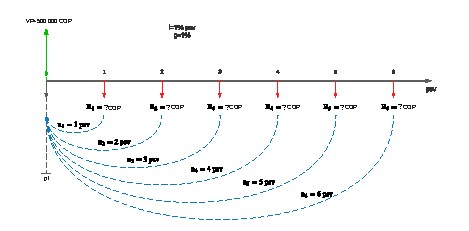
\includegraphics[trim=-78 -5 -78 -5]{7_Capitulo/img/ejemplos/10/10_1.pdf} }   \\ \hline
			%%%%% INICIO FLUJO DE CAJA
			\rowcolor[HTML]{FFB183}
			\multicolumn{2}{|c|}{\cellcolor[HTML]{FFB183}\textbf{4. Declaración de fórmulas}} \\ \hline
			%%%%%%%%%%%%% FIN INSERCIÓN DE IMAGEN
			%%%%%FIN FLUJO DE CAJA
			
			\multicolumn{2}{|c|}{ $(1+i_1)^{m_1} = (1+i_2)^{m_2} $ Equivalencia de tasas}   \\  
			\multicolumn{2}{|c|}{ $VF = R\frac{(1+i)^{n} -1 }{i} $ Valor presente serie uniforme}   \\  \hline
			
			%%%%%% INICIO DESARROLLO MATEMÁTICO
			\rowcolor[HTML]{FFB183}
			%%%%%%%%%%INICIO TITULO
			\multicolumn{2}{|c|}{\cellcolor[HTML]{FFB183}\textbf{5. Desarrollo matemático}}       \\ \hline
			%%%%%%%%%% FIN TITULO
			%%%%%%%%%% INICIO MATEMÁTICAS
			\multicolumn{2}{|c|}{  $(1+ 0,24)^{1} = (1+i)^{2} $}   \\ 
			\multicolumn{2}{|c|}{ $  i = 11,3552873\% \hspace{1mm} psv $}   \\  \hline
			
			%%%%%%%%%% FIN MATEMÁTICAS
			%%%%%% FIN DESARROLLO MATEMÁTICO
			%%%%%% INICIO RESPUESTA
			\rowcolor[HTML]{FFB183}
			%%%%%%%%%%INICIO TITULO
			\multicolumn{2}{|c|}{\cellcolor[HTML]{FFB183}\textbf{6. Respuesta}}   \\ \hline
			%%%%%%%%%% FIN TITULO
			%%%%%%%%%% INICIO RESPUESTA MATEMÁTICA
			\multicolumn{2}{|c|}{ 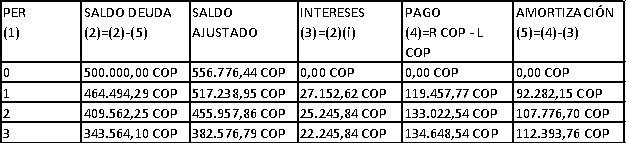
\includegraphics[trim=-78 -5 -78 -5]{7_Capitulo/img/ejemplos/10/10_2.pdf} }   \\ \hline
			%\multicolumn{2}{|C{\textwidth}|}{
			%	$R_{58} = 72.478,16 \ COP (1 + 0,02)^{57} = \ COP 224.087,15 $ 
			%}  \\ \hline
			
			
			%%%%%%%%%% FIN MATEMÁTICAS
			%%%%%% FIN RESPUESTA
		\end{longtable}
		%Se crean dos lineas en blanco para que no quede el siguiente texto tan pegado
		%\newline \newline %USARLO SI CREES QUE ES NECESARIO
	\end{center}
 %%%%%%%%%%%%%%%%%%%%%%%%%%FIN EJERCICIO 10 %%%%%%%%%%%%%%%%%%%%%%%%%%%

\section{Ecuaciones de equivalencia de flujos}
Es muy frecuente cambiar una o varias obligaciones por otra u otras nuevas obligaciones. La solución de este problema es elemental y para solucionarlo es necesario usar la ecuación de equivalencia de flujos, que es una igualdad de valores ubicados en una sola fecha denominada período focal.\\
La período focal se representa gráficamente por una línea a trazos y por las letras pf y es la fecha en que debe hacerse la igualdad entre ingresos (flujos positivos) y egresos (flujos negativos) . La ubicación de la período focal no altera la respuesta final, por tal motivo se deja a libre elección de la persona que va a resolver el problema.\\
El principio fundamental de una ecuación de valor, que viene a ser el mismo principio fundamental de las finanzas, establece que la sumatoria de los ingresos debe ser igual a la sumatoria de los egresos ubicados ambos en la período focal, esto es:

\begin{center}
   $\sum ingresos = \sum egresos(en\ la\ pf)$\\
\end{center}
Naturalmente, para el traslado de cada una de las cantidades a la período focal, debe hacerse usando la fórmula de valor futuro.\\
El enunciado de una ecuación de equivalencia también puede ser expresado así:

\begin{center}
   $\sum deudas = \sum pagos(en\ la\ pf)$\\
\end{center}

Mirando un balance el principio puede ser expresado así:\\

\begin{center}
   $\sum activos = \sum pasivos + capital(en\ la\ pf)$\\
\end{center}

Como en cualquier proyecto, los ingresos se representan por flechas hacia arriba y los egresos por flechas hacia abajo, entonces, mirando la gráfica de flujo de caja podemos expresar el principio fundamental de una ecuación de equivalencia de flujos de esta otra forma:\\

\begin{center}
   $\sum de\ lo\ que\ $\textit{está}$\ para\ arriba = \sum de\ lo\ que\ $\textit{está}$\ para\ abajo(en\ la\ pf)$\\
\end{center}

La sumatoria de los ingresos en pesos de hoy menos la sumatoria de los egresos en pesos de hoy recibe el nombre de valor presente neto (VPN) o valor actual neto.\\
La tasa a la cual la sumatoria de los ingresos (VPN) es igual a la sumatoria de los egresos (en la período focal) se denomina tasa interna de retorno (TIR).\\
En el capítulo posterior analizaremos con más detalle los conceptos de VPN y TIR, estos conceptos son de suma importancia en la evaluación de proyectos.\\

\textbf{Ejemplo 11}\\
Hallar el valor presente de 15 pagos que decrecen
linealmente en 400 COP, si el primer pago es de 5.000 COP y la tasa efectiva es del 4\% período año
vencido..\\ \\
%\newpage %USAR SOLO SI EL SOLUCIÓN QUEDA SOLO Y ES NECESARIO BAJARLO A LA SIGUIENTE PAGINA
\textbf{Solución.}\\
%La tabla ira centrada
\begin{center}
 \renewcommand{\arraystretch}{1.5}% Margenes de las celdas
 %Creación de la cuadricula de 3 columnas
 \begin{longtable}[H]{|p{0.5\linewidth}|p{0.5\linewidth}|}
  \hline
  \multicolumn{2}{|c|}{\cellcolor[HTML]{FFB183}\textbf{1. Declaración de variables}}                                                                                                                 \\ \hline
  $R =  5.400 COP$                                                                                & $L = 400 COP$                                                                                   \\
  $n=15 \hspace{1mm} pav$                                                                         & $VP=? COP$                                                                                         \\
  $i=4,0\% \hspace{1mm} pav$                                                                      &                                                                                                  \\
  \multicolumn{2}{|c|}{\cellcolor[HTML]{FFB183}\textbf{2. Diagrama de flujo de caja}}                                                                                                                \\ \hline
  \multicolumn{1}{|c|}{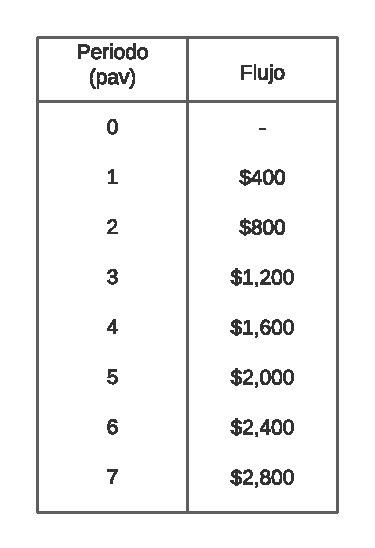
\includegraphics[trim=-5 -5 -5 -5 ,width=0.5\columnwidth]{11/Tabla 1.pdf}} & \multicolumn{1}{|c|}{ 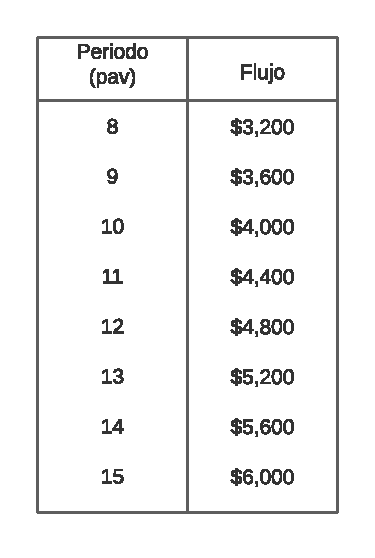
\includegraphics[trim=-5 -5 -5 -5 ,width=0.5\columnwidth]{11/Tabla 2.pdf}} \\ \hline
  \multicolumn{2}{|c|}{\cellcolor[HTML]{FFB183}\textbf{3. Aplicación de funciones}}                                                                                                                  \\ \hline
  \multicolumn{2}{|p{\columnwidth}|}{Se aplicará la función valor presente VNA de la siguiente forma: \newline
  =VNA(0,04;J8::J22) con referencia en la hoja de
  Excel usada para el ejercicio.}                                                                                                                                                                    \\
  \multicolumn{2}{|c|}{ 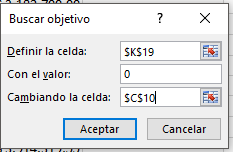
\includegraphics[trim=-5 -5 -5 -5 ,width=0.7\columnwidth]{11/excel1.png}}                                                                                                    \\ \hline
  \multicolumn{2}{|c|}{\cellcolor[HTML]{FFB183}\textbf{4. Gráfica}}                                                                                                                                  \\ \hline
  \multicolumn{2}{|c|}{ \includegraphics[trim=-5 -5 -5 -5 ,width=0.8\columnwidth]{11/gráfico.pdf}}                                                                                                   \\ \hline
  \multicolumn{2}{|c|}{\cellcolor[HTML]{FFB183}\textbf{5. Respuesta}}                                                                                                                                \\ \hline
  \multicolumn{2}{|c|}{El valor presente es VP =  COP 27.697,9410}                                                                                                                                      \\ \hline
 \end{longtable}
 %\newline \newline %USARLO SI CREES QUE ES NECESARIO
\end{center}


\textbf{Ejemplo 12}\\
Hallar el valor presente de una serie infinita de egresos que crecen en un 10\%, si la tasa de interés es del 20\% pav y el primer egreso es  300.000COP.\\


%%%%%%%%%%%%%%%%%%% EJERCICIO 12 %%%%%%

%\newpage %USAR SOLO SI EL SOLUCIÓN QUEDA SOLO Y ES NECESARIO BAJARLO A LA SIGUIENTE PAGINA
\textbf{Solución.}\\
%La tabla ira centrada
\begin{center}
	\renewcommand{\arraystretch}{1.6}% Margenes de las celdas
	%Creación de la cuadricula de 3 columnas
	\begin{longtable}[H]{|c|c|c|}
		%Creamos una linea horizontal
		\hline
		%Definimos el color de la primera fila
		\rowcolor[HTML]{FFB183}
		%%%%% INICIO ASIGNACIÓN FECHA FOCAL %%%%%%%
		%%%%%%%%%% INICIO TITULO
		%Lo que se hace aquí es mezclar las 3 columnas en una sola
		\multicolumn{3}{|c|}{\cellcolor[HTML]{FFB183}\textbf{1. Asignación período focal}}  \\ \hline
		\multicolumn{3}{|c|}{$pf = \textit{0 pav}$}   \\\hline
		%%%%%%%%%% FIN TITULO
		%%%%% INICIO DECLARACIÓN DE VARIABLES %%%%%%%
		%%%%%%%%%% INICIO TITULO
		%Lo que se hace aquí es mezclar las 3 columnas en una sola
		\multicolumn{3}{|c|}{\cellcolor[HTML]{FFB183}\textbf{2. Declaración de variables}}   \\ \hline
		%%%%%%%%%% FIN TITULO
		%%%%%%%%%% INICIO DE MATEMÁTICAS
		%Cada & hace referencia al paso de la siguiente columna
		\multicolumn{2}{|c|}{\textbf{$\hspace{3.5 cm}\textit{}\hspace{3.5 cm}$}} & \textbf{$\hspace{3.5 cm}\textit{}\hspace{3.5 cm}$} \\ 
		\multicolumn{2}{|c|}{$\hspace{2 cm}R=  300{.}000COP \hspace{2 cm}$} & $i=20\% \textit{ pav}$ \\
		\multicolumn{2}{|c|}{$\hspace{2 cm}n_1=10  \textit{ pav} \hspace{2 cm}$} & $g=10\% \textit{creciente entre flujos} $ \\
		\multicolumn{2}{|c|}{$\hspace{2 cm}VF= ?COP \hspace{2 cm}$} &  \\ \hline	
		
		%%%%%%%%%% FIN DE MATEMÁTICAS
		%%%%% FIN DECLARACIÓN DE VARIABLES
		
		%%%%% INICIO FLUJO DE CAJA
		\rowcolor[HTML]{FFB183}
		\multicolumn{3}{|c|}{\cellcolor[HTML]{FFB183}\textbf{3. Diagrama de flujo de caja}} \\ \hline
		%Mezclamos 3 columnas y pondremos el dibujo
		%%%%%%%%%%%%% INSERCIÓN DE LA IMAGEN
		%Deberán descargar las imágenes respectivas del drive y pegarlas en la carpeta
		%n_capitulo/img/ejemplos/1/capitulo1ejemplo1.pdf  (el /1/ es el numero del ejemplo)
		\multicolumn{3}{|c|}{ 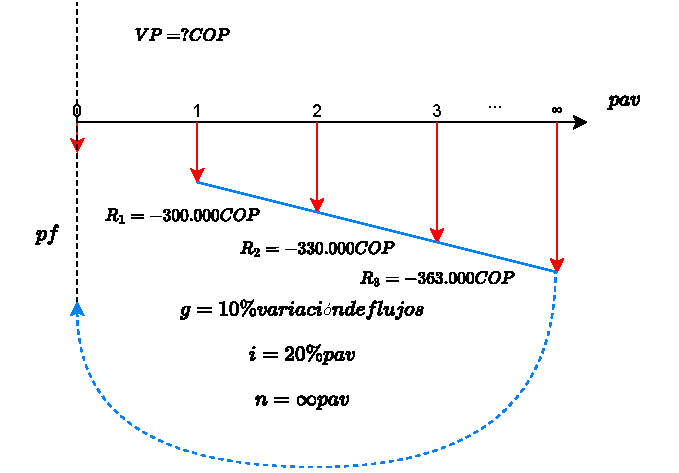
\includegraphics[trim=-5 -5 -5 -5 , scale=0.9]{6_Capitulo/img/ejemplos/12/Capitulo6Ejemplo12.pdf} }
		\\ \hline
		%%%%%%%%%%%%% FIN INSERCIÓN DE IMAGEN
		%%%%%FIN FLUJO DE CAJA
		
		%%%%% INICIO DECLARACIÓN FORMULAS
		%%%%%%%%%%% INICIO TITULO
		\rowcolor[HTML]{FFB183}
		\multicolumn{3}{|c|}{\cellcolor[HTML]{FFB183}\textbf{4. Declaración de fórmulas}}    \\ \hline
		%%%%%%%%%%% FIN TITULO
		%%%%%%%%%%% INICIO MATEMÁTICAS
		\multicolumn{3}{|c|}{$VP=(\frac{R}{i-g}) \hspace{0.4 cm} \textit{Valor gradiente si geométrico infinito si g<1} $} \\   \hline
		
		%%%%%%%%%% FIN MATEMÁTICAS
		%%%%%% INICIO DESARROLLO MATEMÁTICO
		\rowcolor[HTML]{FFB183}
		%%%%%%%%%%INICIO TITULO
		\multicolumn{3}{|c|}{\cellcolor[HTML]{FFB183}\textbf{5. Desarrollo matemático}}       \\ \hline
		%%%%%%%%%% FIN TITULO
		%%%%%%%%%% INICIO MATEMÁTICAS
		\multicolumn{3}{|c|}{$VP=(\frac{  300{.}000COP}{0.2-0.1}) \hspace{0.2 cm}\rightarrow \hspace{0.2 cm} VP= 300{.}000 COP$} \\  \hline
		%%%%%%%%%% FIN MATEMÁTICAS
		%%%%%% FIN DESARROLLO MATEMÁTICO
		%%%%%% INICIO RESPUESTA
		\rowcolor[HTML]{FFB183}
		%%%%%%%%%%INICIO TITULO
		\multicolumn{3}{|c|}{\cellcolor[HTML]{FFB183}\textbf{6. Respuesta}}   \\ \hline
		%%%%%%%%%% FIN TITULO
		%%%%%%%%%% INICIO RESPUESTA MATEMÁTICA
		\multicolumn{3}{|c|}{${VP=  300.000 COP }$} \\ \hline
		%%%%%%%%%% FIN MATEMÁTICAS
		%%%%%% FIN RESPUESTA
	\end{longtable}
	%Se crean dos lineas en blanco para que no quede el siguiente texto tan pegado
	%\newline \newline %USARLO SI CREES QUE ES NECESARIO
\end{center}

%%%%%%%%%%%%%%%%%%%%%%%%%%FIN EJERCICIO 12 %%%%%%%%%%%%%%%%%%%%%%%%%%%

	%%%%%%%%%%%%%%%%%%%%%%%%%%EJERCICIO 13 %%%%%%%%%%%%%%%%%%%%%%%%%%%%%%%%%%%%%%%%%%%%%%%%%%%%%%
    \textbf{Ejemplo 13}\\
	
	Una cuota inicial del 30\% y el saldo será pagadero al final de 3 años, mientras tanto se pagarán intereses por período mes anticipado al 3\%. Con el objeto de cancelar la deuda a su vencimiento, se constituye un fondo que paga el 33\% nominal anual mes vencido mediante depósitos mensuales ordinarios crecientes en 2.000 COP. Determinar el costo del período 15.\\
	
	\textbf{Solución 13}\\
	%La tabla ira centrada
	\begin{center}
		\renewcommand{\arraystretch}{1.5}% Margenes de las celdas
		%Creación de la cuadricula de 3 columnas
		\begin{longtable}[H]{|p{0.5\linewidth}|p{0.5\linewidth}|}
			%Creamos una linea horizontal
			\hline
			%Definimos el color de la primera fila
			\rowcolor[HTML]{FFB183}
			%%%%% INICIO ASIGNACIÓN período FOCAL %%%%%%%
			%%%%%%%%%% INICIO TITULO
			%Lo que se hace aquí es mezclar las 3 columnas en una sola
			\multicolumn{2}{|c|}{\cellcolor[HTML]{FFB183}\textbf{1. Asignación período focal}}   \\ \hline
			%%%%%%%%%% FIN TITULO
			%%%%% INICIO DECLARACIÓN DE VARIABLES %%%%%%%
			\multicolumn{2}{|c|}{$pf = 36 \textit{ pmv}$}\\ \hline
			%%%%%%%%%% INICIO TITULO
			%Lo que se hace aquí es mezclar las 3 columnas en una sola
			\multicolumn{2}{|c|}{\cellcolor[HTML]{FFB183}\textbf{2. Declaración de variables}}   \\ \hline
			%%%%%%%%%% FIN TITULO
			%%%%%%%%%% INICIO DE MATEMÁTICAS
			%Cada & hace referencia al paso de la siguiente columna
			$  Interés = 4.200.000 \ COP (0,03) = 126.000 \ COP $  			 \\ \hline
			%%%%%%%%%% FIN DE MATEMÁTICAS
			%%%%% FIN DECLARACIÓN DE VARIABLES
			
			\rowcolor[HTML]{FFB183}
			\multicolumn{2}{|c|}{\cellcolor[HTML]{FFB183}\textbf{3. Diagrama de flujo de caja}} \\ \hline
			\multicolumn{2}{|c|}{ 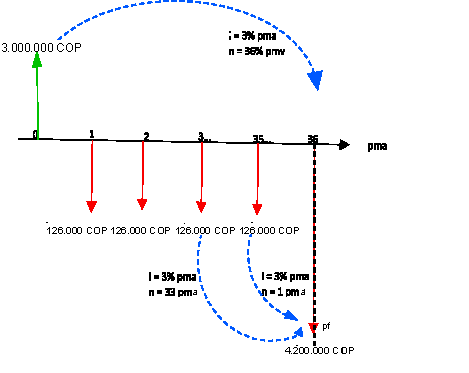
\includegraphics[trim=-78 -5 -78 -5]{7_Capitulo/img/ejemplos/13/13_1.pdf} }   \\
			\multicolumn{2}{|c|}{ 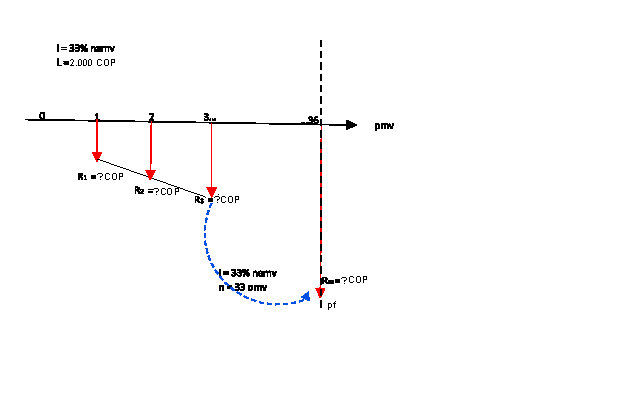
\includegraphics[trim=-78 -5 -78 -5]{7_Capitulo/img/ejemplos/13/13_2.pdf} }   \\ \hline
			%%%%% INICIO FLUJO DE CAJA
			\rowcolor[HTML]{FFB183}
			\multicolumn{2}{|c|}{\cellcolor[HTML]{FFB183}\textbf{4. Declaración de fórmulas}} \\ \hline
			%%%%%%%%%%%%% FIN INSERCIÓN DE IMAGEN
			%%%%%FIN FLUJO DE CAJA
			\multicolumn{2}{|c|}{ $VF = R n(1+i)^{n-1} $ \hspace{1mm} Formula del valor futuro gradiente geométrico si g=i}\\    
			\multicolumn{2}{|c|}{ $R_{n} = R_{1} + (n-1)L $ \hspace{1mm} Valor de un periodo aritmetico en un periodo n}   \\ \hline
			
			%%%%%% INICIO DESARROLLO MATEMÁTICO
			\rowcolor[HTML]{FFB183}
			%%%%%%%%%%INICIO TITULO
			\multicolumn{2}{|c|}{\cellcolor[HTML]{FFB183}\textbf{5. Desarrollo matemático}}       \\ \hline
			%%%%%%%%%% FIN TITULO
			%%%%%%%%%% INICIO MATEMÁTICAS
			\multicolumn{2}{|c|}{  $ 4.200.000 \ COP = R_{1} (36) (0,0275) + \frac{ 2.000 \ COP }{0,0275} ((36)(0,0275)-36) $}   \\ 
			\multicolumn{2}{|c|}{  $  R_{1} = 40.531,73 \ COP $}   \\ 
			\multicolumn{2}{|c|}{ $  R_{15} = 40.531,73 \ COP +  ( 15 - 1) (2.000 \ COP) = 68.531,73 \ COP $}   \\  \hline
			
			%%%%%%%%%% FIN MATEMÁTICAS
			%%%%%% FIN DESARROLLO MATEMÁTICO
			%%%%%% INICIO RESPUESTA
			\rowcolor[HTML]{FFB183}
			%%%%%%%%%%INICIO TITULO
			\multicolumn{2}{|c|}{\cellcolor[HTML]{FFB183}\textbf{6. Respuesta}}   \\ \hline
			%%%%%%%%%% FIN TITULO
			%%%%%%%%%% INICIO RESPUESTA MATEMÁTICA
			%\multicolumn{2}{|c|}{ 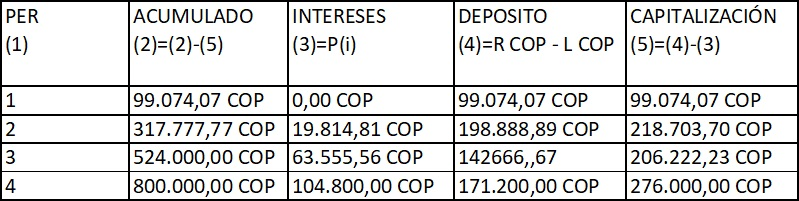
\includegraphics[trim=-78 -5 -78 -5]{7_Capitulo/img/ejemplos/12/12_2.jpg} }   \\ \hline
			\multicolumn{2}{|C{\textwidth}|}{
				$  R_{1} = 40.531,73 \ COP \hspace{2mm} y  \hspace{2mm} R_{15} = 68.531,73 \ COP $
				
				Esto significa que en el período 15 el deudor debe disponer de 194.531,73 COP de los cuales 126.000 COP los dedica al pago de intereses y el resto (68.531,73 COP) se deposita en el fondo.
				
			}  \\ \hline
			
			
			%%%%%%%%%% FIN MATEMÁTICAS
			%%%%%% FIN RESPUESTA
		\end{longtable}
		%Se crean dos lineas en blanco para que no quede el siguiente texto tan pegado
		%\newline \newline %USARLO SI CREES QUE ES NECESARIO
	\end{center}
%%%%%%%%%%%%%%%%%%%%%%%%%%FIN EJERCICIO 13
%%%%%%%%%%%%%%%%%%%% EJERCICIO 14 %%%%%%

\textbf{Ejemplo 14}\\
Una persona debe pagar 70.000 COP en 3 meses y 85.000 COP en 8 meses; ante la imposibilidad de cancelar las deudas en las fechas previstas le ofrece al acreedor que le cancelara 50.000 COP en 4 meses y 130.000 COP en 12 meses. Si el acreedor acepta esta nueva forma de pago ¿Qué tasa de interés periódica mes vencido estará pagando?.\\ \\
\setlength{\parskip}{-1mm}
%\newpage %USAR SOLO SI EL SOLUCIÓN QUEDA SOLO Y ES NECESARIO BAJARLO A LA SIGUIENTE PAGINA
\textbf{Solución.}
%La tabla ira centrada

\begin{center}
  \renewcommand{\arraystretch}{1.5}% Margenes de las celdas
  %Creación de la cuadricula de 3 columnas
  \begin{longtable}[H]{|c|c|c|}
    %Creamos una linea horizontal
    \hline
    %Definimos el color de la primera fila
    \rowcolor[HTML]{FFB183}
    %%%%% INICIO ASIGNACIÓN PERíODO FOCAL %%%%%%%
    %%%%%%%%%% INICIO TITULO
    %Lo que se hace aquí es mezclar las 3 columnas en una sola
    \multicolumn{3}{|c|}{\cellcolor[HTML]{FFB183}\textbf{1. Asignación período focal}}                                                      \\ \hline
    \multicolumn{3}{|c|}{\textbf{ $pf = \textit{ período focal: 0 pmv} $}}                                                                  \\ \hline
    %%%%%%%%%% FIN TITULO
    %%%%% INICIO DECLARACIÓN DE VARIABLES %%%%%%%
    %%%%%%%%%% INICIO TITULO
    %Lo que se hace aquí es mezclar las 3 columnas en una sola
    \multicolumn{3}{|c|}{\cellcolor[HTML]{FFB183}\textbf{2. Declaración de variables}}                                                      \\ \hline
    %%%%%%%%%% FIN TITULO
    %%%%%%%%%% INICIO DE MATEMÁTICAS
    %Cada & hace referencia al paso de la siguiente columna
    $F_{1} =    70.000  $ COP & $F_{3} =    50.000 $  COP  & $n_ {2} = -8 \textit{ pmv}  $                                                  \\
    $F_{2} =    85.000  $ COP & $F_{4} =    130.000  $ COP & $n_ {3} = -4 \textit{ pmv}   $                                                 \\
    $i = ?\%  $               & $n_{1} = -3 \textit{ pmv}  $ & $n_ {4} = -12 \textit{ pmv}  $                                                 \\ \hline

    %%%%%%%%%% FIN DE MATEMÁTICAS
    %%%%% FIN DECLARACIÓN DE VARIABLES


    %%%%% INICIO FLUJO DE CAJA
    \rowcolor[HTML]{FFB183}
    \multicolumn{3}{|c|}{\cellcolor[HTML]{FFB183}\textbf{3. Diagrama de flujo de caja}}                                                     \\ \hline
    %Mezclamos 3 columnas y pondremos el dibujo
    %%%%%%%%%%%%% INSERCIÓN DE LA IMAGEN
    %Deberán descargar las imágenes respectivas del drive y pegarlas en la carpeta
    %n_capitulo/img/ejemplos/1/capitulo1ejemplo1.pdf  (el /1/ es el numero del ejemplo)
    \multicolumn{3}{|c|}{ 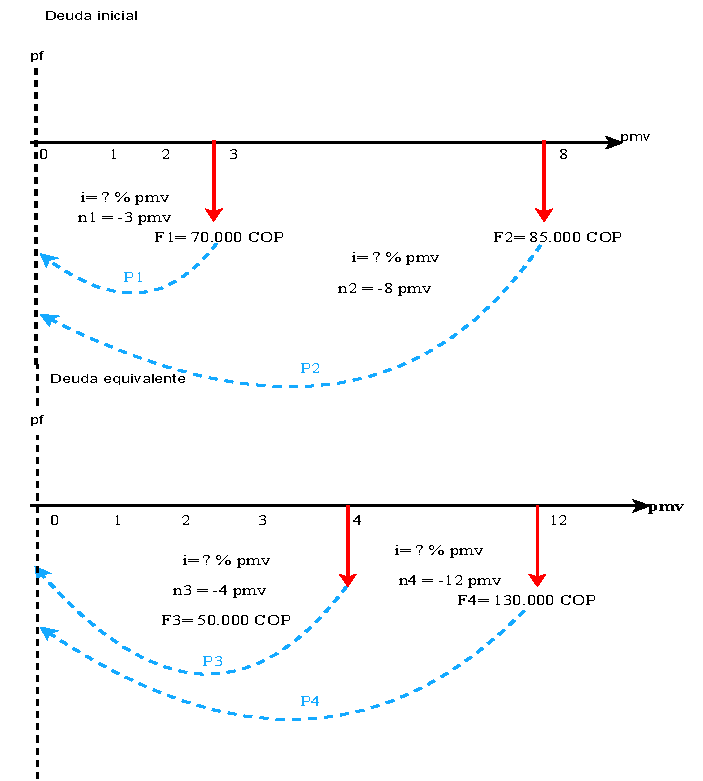
\includegraphics[trim=-5 -5 -5 -5 , scale=0.65]{2_Capitulo/img/ejemplos/14/Ejemplo 14Ver.pdf} } 
    \ \\ \hline
    %%%%%%%%%%%%% FIN INSERCIÓN DE IMAGEN
    %%%%%FIN FLUJO DE CAJA



    %%%%% INICIO DECLARACIÓN FORMULAS
    %%%%%%%%%%% INICIO TITULO
    \rowcolor[HTML]{FFB183}
    \multicolumn{3}{|c|}{\cellcolor[HTML]{FFB183}\textbf{4. Declaración de fórmulas}}                                                       \\ \hline
    %%%%%%%%%%% FIN TITULO
    %%%%%%%%%%% INICIO MATEMÁTICAS

    \multicolumn{3}{|c|}{$P = F(1+i)^{-n} \hspace{0.3cm} \textit{Valor presente }$}                                                         \\
    \multicolumn{3}{|c|}{$P_{1} + P_{2} = P_{3} + P_{4} \hspace{0.3cm} \textit{Ecuación de eqv.}$ }                                         \\
    \hline
    %%%%%%%%%% FIN MATEMÁTICAS
    %%%%%% INICIO DESARROLLO MATEMÁTICO
    \rowcolor[HTML]{FFB183}
    %%%%%%%%%%INICIO TITULO
    \multicolumn{3}{|c|}{\cellcolor[HTML]{FFB183}\textbf{5. Desarrollo matemático}}                                                         \\ \hline
    %%%%%%%%%% FIN TITULO
    %%%%%%%%%% INICIO MATEMÁTICAS


    \multicolumn{3}{|c|}{$ 70.000$ COP $(1+i)^{-3}  + 85.000$ COP $(1+i)^{-8}$}
    \\
    \multicolumn{3}{|c|}{$=50.000$ COP $(1+i)^{-4} + 130.000$ COP $(1+i)^{-12}$}      \\
    \multicolumn{3}{|c|}{$ 70(1+i)^{-3} +85(1+i)^{-8} - 50(1+i)^{-4} - 130(1+i)^{-12} = 0   $ }                                             \\
    \multicolumn{3}{|c|}{$ \textit{Primer ensayo:} $ }                                                                                      \\
    \multicolumn{3}{|c|}{$ i_{1} = 2\% \textit{ pmv} $ }                                                                                    \\
    \multicolumn{3}{|c|}{$70$ COP $(1+0,02)^{-3} +85$ COP $(1+0,02)^{-8}$} 
    \\
    \multicolumn{3}{|c|} {$-50$ COP $(1+0,02)^{-4} - 130$  COP $(1+0,02)^{-12} = -10.18714 $ } \\
    \multicolumn{3}{|c|}{$ \textit{Segundo ensayo:} $ }                                                                                     \\
    \multicolumn{3}{|c|}{$ i_{2} = 3\% \textit{ pmv} $ }                                                                                    \\
    \multicolumn{3}{|c|}{$ 70$ COP $(1+0,03)^{-3} +85$ COP $(1+0,03)^{-8}$}
    \\
    \multicolumn{3}{|c|}{$-50$ COP $(1+0,03)^{-4} -130$ COP $(1+0,03)^{-12} = -4,44404 $ }   \\
    \multicolumn{3}{|c|}{$ \textit{Tercer ensayo:} $ }                                                                                      \\
    \multicolumn{3}{|c|}{$ i_{3} = 4\% \textit{ pmv} $ }                                                                                    \\
    \multicolumn{3}{|c|}{$70$ COP $(1+0,04)^{-3} +85$ COP $(1+0,04)^{-8}$}
    \\
    \multicolumn{3}{|c|}{$-50$ COP $(1+0,04)^{-4} -130$ COP $(1+0,04)^{-12} = 0.400587 $ }
    \\
    
    \multicolumn{3}{|c|}{$ 	\textit{ Se toman los resultados correspondientes al 3\% y a 4\% por ser los más cercanos y} $ }                 \\
    \multicolumn{3}{|c|}{$ 	\textit{los que presentan diferente signo y los colocaremos de la siguiente forma:} $ }                          \\
    \multicolumn{3}{|c|}{$ \textit{ Se plantea una proporción, teniendo en cuenta las diferencias mostradas en los} $ }                     \\
    \multicolumn{3}{|c|}{$ \textit{corchetes y siempre manteniendo el mismo orden.} $ }                                                     \\
    \multicolumn{3}{|c|}{$ \frac{3-i}{3-4} = \frac{-4,44404-0}{-4,44404-0,400587}$ }                                                                \\ \hline


    %%%%%%%%%% FIN MATEMÁTICAS
    %%%%%% FIN DESARROLLO MATEMÁTICO
    %%%%%% INICIO RESPUESTA
    \rowcolor[HTML]{FFB183}
    %%%%%%%%%%INICIO TITULO
    \multicolumn{3}{|c|}{\cellcolor[HTML]{FFB183}\textbf{6. Respuesta}}                                                                     \\ \hline
    %%%%%%%%%% FIN TITULO
    %%%%%%%%%% INICIO RESPUESTA MATEMÁTICA
    \multicolumn{3}{|c|}{

      \begin{minipage}[t][0.07\textheight][c]{0.8\columnwidth}
       \centering
        $i = 3,917313\% \textit{ pmv}$ .
      \end{minipage}
    }                                                                                                                                       \\ \hline


    %%%%%%%%%% FIN MATEMÁTICAS
    %%%%%% FIN RESPUESTA
  \end{longtable}
  %Se crean dos lineas en blanco para que no quede el siguiente texto tan pegado
  %\newline \newline %USARLO SI CREES QUE ES NECESARIO
\end{center}
%%%%%%%%%%%%%%%%%%%%%%%%%%FIN EJERCICIO 14 %%%%%%%%%%%%%%%%%%%%%%%%%%%
%%%%%%%%%%%%%%%%%%%% EJERCICIO 15 %%%%%%

\textbf{Ejemplo 15}\\
Una persona debe pagar  COP  100,000 con vencimiento en 3 meses,  COP  150,000 a 10 meses y
COP  200,000 con vencimiento en un año. Si hace un pago único de  COP  450,000, hallar la fecha en
que debe hacerse, suponga una tasa del 18\% nominal anual mes vencido.
Si consideramos la período focal (pf) en el período mes vencido 12:\\ \\

%\newpage %USAR SOLO SI EL SOLUCIÓN QUEDA SOLO Y ES NECESARIO BAJARLO A LA SIGUIENTE PAGINA
\textbf{Solución.}\\
%La tabla ira centrada
\begin{center}
  \renewcommand{\arraystretch}{1.5}% Margenes de las celdas
  %Creación de la cuadricula de 3 columnas
  \begin{longtable}[H]{|c|c|c|}
    %Creamos una linea horizontal
    \hline
    %Definimos el color de la primera fila
    \rowcolor[HTML]{FFB183}
    %%%%% INICIO ASIGNACIÓN PERíODO FOCAL %%%%%%%
    %%%%%%%%%% INICIO TITULO
    %Lo que se hace aquí es mezclar las 3 columnas en una sola
    \multicolumn{3}{|c|}{\cellcolor[HTML]{FFB183}\textbf{1. Asignación período focal}}                                                                                          \\ \hline
    \multicolumn{3}{|c|}{\textbf{ $pf = \textit{ período focal: 0 pmv} $}}                                                                                                      \\ \hline
    %%%%%%%%%% FIN TITULO
    %%%%% INICIO DECLARACIÓN DE VARIABLES %%%%%%%
    %%%%%%%%%% INICIO TITULO
    %Lo que se hace aquí es mezclar las 3 columnas en una sola
    \multicolumn{3}{|c|}{\cellcolor[HTML]{FFB183}\textbf{2. Declaración de variables}}                                                                                          \\ \hline
    %%%%%%%%%% FIN TITULO
    %%%%%%%%%% INICIO DE MATEMÁTICAS
    %Cada & hace referencia al paso de la siguiente columna

    $j = 18\% \textit{ namv} $                                 & $P_{1} =  COP  100.000  $                                                      & $n_{1} = 9 \textit{ pmv} $    \\
    $i = 1,5\% \textit{ pmv} $                                 & $P_{2} =  COP  150.000  $                                                      & $n_{2} = 2 \textit{ pmv} $    \\
                                                               & $P_{3} =  COP  200.000  $                                                      & $n_{3}= 0 \textit{ pmv}  $    \\
                                                               & $p_{4} =  COP  450.000  $                                                      & $n_{4} = 12-n \textit{ pmv} $ \\ \hline

    %%%%%%%%%% FIN DE MATEMÁTICAS
    %%%%% FIN DECLARACIÓN DE VARIABLES


    %%%%% INICIO FLUJO DE CAJA
    \rowcolor[HTML]{FFB183}
    \multicolumn{3}{|c|}{\cellcolor[HTML]{FFB183}\textbf{3. Diagrama de flujo de caja}}                                                                                         \\ \hline
    %Mezclamos 3 columnas y pondremos el dibujo
    %%%%%%%%%%%%% INSERCIÓN DE LA IMAGEN
    %Deberán descargar las imágenes respectivas del drive y pegarlas en la carpeta
    %n_capitulo/img/ejemplos/1/capitulo1ejemplo1.pdf  (el /1/ es el numero del ejemplo)
    \multicolumn{3}{|c|}{ 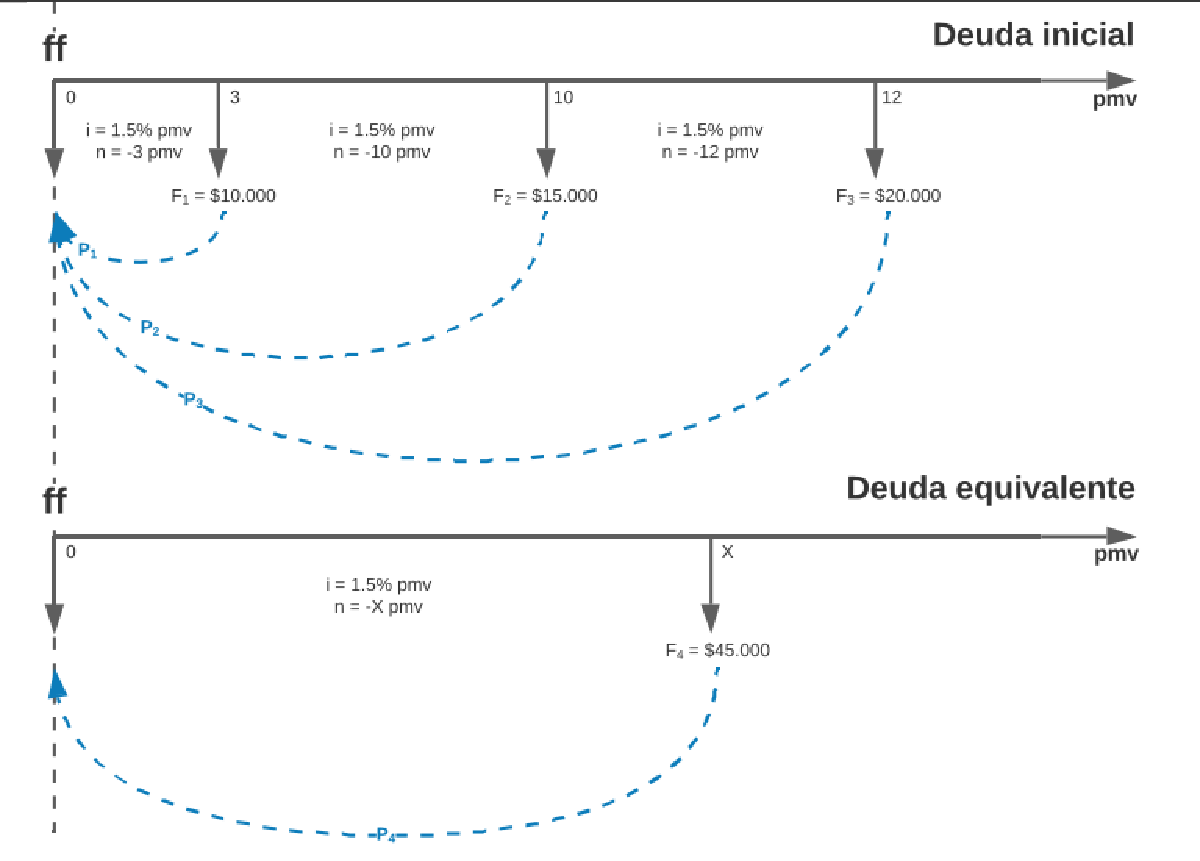
\includegraphics[trim=-5 -5 -5 -5 , scale=0.64]{14/Capitulo2Ejercicio15.pdf} }
    \\ \hline
    %%%%%%%%%%%%% FIN INSERCIÓN DE IMAGEN
    %%%%%FIN FLUJO DE CAJA



    %%%%% INICIO DECLARACIÓN FORMULAS
    %%%%%%%%%%% INICIO TITULO
    \rowcolor[HTML]{FFB183}
    \multicolumn{3}{|c|}{\cellcolor[HTML]{FFB183}\textbf{4. Declaración de fórmulas}}                                                                                           \\ \hline
    %%%%%%%%%%% FIN TITULO
    %%%%%%%%%%% INICIO MATEMÁTICAS

    $P_{1} + P_{2} + P_{3} = P_{4} \textit{ Ecuación de eqv.}$ & \multicolumn{2}{c|}{$P = F(1+i)^(-n) \hspace{0.3cm} \textit{Valor presente}$ }                                 \\
                                                               & \multicolumn{2}{c|}{$F = P(1+i)^n \hspace{0.3cm} \textit{Valor futuro}$   }                                    \\ \hline
    %%%%%%%%%% FIN MATEMÁTICAS
    %%%%%% INICIO DESARROLLO MATEMÁTICO
    \rowcolor[HTML]{FFB183}
    %%%%%%%%%%INICIO TITULO
    \multicolumn{3}{|c|}{\cellcolor[HTML]{FFB183}\textbf{5. Desarrollo matemático}}                                                                                             \\ \hline
    %%%%%%%%%% FIN TITULO
    %%%%%%%%%% INICIO MATEMÁTICAS

    \multicolumn{3}{|C{\linewidth}|}{$  COP  100.000( 1 + 0,015)^(-3) +  COP  150.000( 1 + 0,015)^(-10) +  COP  200.000( 1 + 0,015)^(-12)= COP  450.000( 1 + 0,015)^(-x) $}     \\
    \multicolumn{3}{|C{\linewidth}|}{$ ln(306.090,07391/450.000)= (-x)ln(1,015)  $ }                                                                                            \\ \hline


    %%%%%%%%%% FIN MATEMÁTICAS
    %%%%%% FIN DESARROLLO MATEMÁTICO
    %%%%%% INICIO RESPUESTA
    \rowcolor[HTML]{FFB183}
    %%%%%%%%%%INICIO TITULO
    \multicolumn{3}{|c|}{\cellcolor[HTML]{FFB183}\textbf{6. Respuesta}}                                                                                                         \\ \hline
    %%%%%%%%%% FIN TITULO
    %%%%%%%%%% INICIO RESPUESTA MATEMÁTICA
    \multicolumn{3}{|c|}{

      \begin{minipage}[t][0.07\textheight][c]{0.8\columnwidth}
        $n_{4} = 9,24059 \textit{ pmv} \approx t = 9 \textit{ meses y }  7 \textit{ dias.} $
      \end{minipage}
    }                                                                                                                                                                           \\ \hline


    %%%%%%%%%% FIN MATEMÁTICAS
    %%%%%% FIN RESPUESTA
  \end{longtable}
  %Se crean dos lineas en blanco para que no quede el siguiente texto tan pegado
  %\newline \newline %USARLO SI CREES QUE ES NECESARIO
\end{center}
%%%%%%%%%%%%%%%%%%%%%%%%%%FIN EJERCICIO 15 %%%%%%%%%%%%%%%%%%%%%%%%%%%

%%%%%%%%%%%%%%%%%%% EJERCICIO 14 %%%%%%

\textbf{Ejemplo 14}\\
Una persona debe pagar 70.000 COP en 3 meses y 85.000 COP en 8 meses; ante la imposibilidad de cancelar las deudas en las fechas previstas le ofrece al acreedor que le cancelara 50.000 COP en 4 meses y 130.000 COP en 12 meses. Si el acreedor acepta esta nueva forma de pago ¿Qué tasa de interés periódica mes vencido estará pagando?.\\ \\
\setlength{\parskip}{-1mm}
%\newpage %USAR SOLO SI EL SOLUCIÓN QUEDA SOLO Y ES NECESARIO BAJARLO A LA SIGUIENTE PAGINA
\textbf{Solución.}
%La tabla ira centrada

\begin{center}
  \renewcommand{\arraystretch}{1.5}% Margenes de las celdas
  %Creación de la cuadricula de 3 columnas
  \begin{longtable}[H]{|c|c|c|}
    %Creamos una linea horizontal
    \hline
    %Definimos el color de la primera fila
    \rowcolor[HTML]{FFB183}
    %%%%% INICIO ASIGNACIÓN PERíODO FOCAL %%%%%%%
    %%%%%%%%%% INICIO TITULO
    %Lo que se hace aquí es mezclar las 3 columnas en una sola
    \multicolumn{3}{|c|}{\cellcolor[HTML]{FFB183}\textbf{1. Asignación período focal}}                                                      \\ \hline
    \multicolumn{3}{|c|}{\textbf{ $pf = \textit{ período focal: 0 pmv} $}}                                                                  \\ \hline
    %%%%%%%%%% FIN TITULO
    %%%%% INICIO DECLARACIÓN DE VARIABLES %%%%%%%
    %%%%%%%%%% INICIO TITULO
    %Lo que se hace aquí es mezclar las 3 columnas en una sola
    \multicolumn{3}{|c|}{\cellcolor[HTML]{FFB183}\textbf{2. Declaración de variables}}                                                      \\ \hline
    %%%%%%%%%% FIN TITULO
    %%%%%%%%%% INICIO DE MATEMÁTICAS
    %Cada & hace referencia al paso de la siguiente columna
    $F_{1} =    70.000  $ COP & $F_{3} =    50.000 $  COP  & $n_ {2} = -8 \textit{ pmv}  $                                                  \\
    $F_{2} =    85.000  $ COP & $F_{4} =    130.000  $ COP & $n_ {3} = -4 \textit{ pmv}   $                                                 \\
    $i = ?\%  $               & $n_{1} = -3 \textit{ pmv}  $ & $n_ {4} = -12 \textit{ pmv}  $                                                 \\ \hline

    %%%%%%%%%% FIN DE MATEMÁTICAS
    %%%%% FIN DECLARACIÓN DE VARIABLES


    %%%%% INICIO FLUJO DE CAJA
    \rowcolor[HTML]{FFB183}
    \multicolumn{3}{|c|}{\cellcolor[HTML]{FFB183}\textbf{3. Diagrama de flujo de caja}}                                                     \\ \hline
    %Mezclamos 3 columnas y pondremos el dibujo
    %%%%%%%%%%%%% INSERCIÓN DE LA IMAGEN
    %Deberán descargar las imágenes respectivas del drive y pegarlas en la carpeta
    %n_capitulo/img/ejemplos/1/capitulo1ejemplo1.pdf  (el /1/ es el numero del ejemplo)
    \multicolumn{3}{|c|}{ 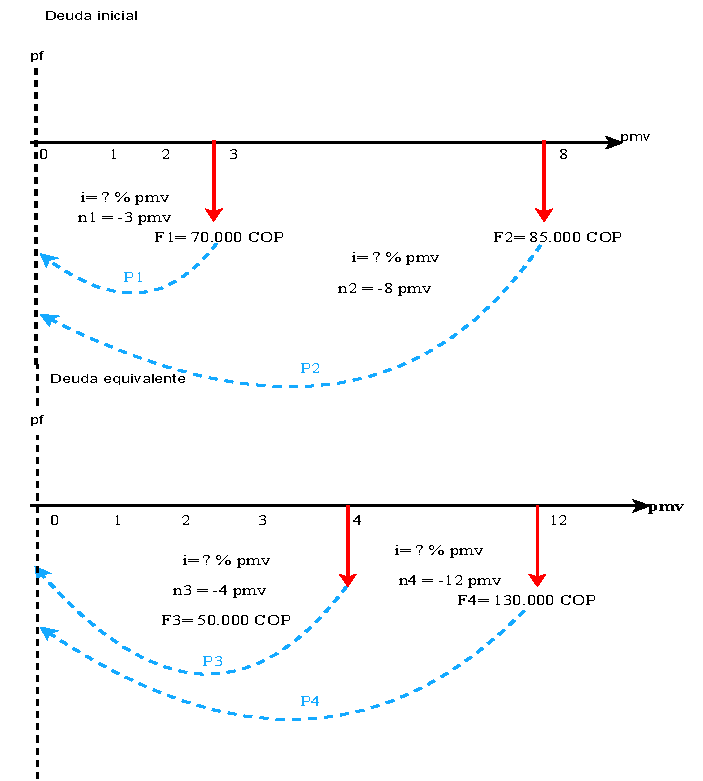
\includegraphics[trim=-5 -5 -5 -5 , scale=0.65]{2_Capitulo/img/ejemplos/14/Ejemplo 14Ver.pdf} } 
    \ \\ \hline
    %%%%%%%%%%%%% FIN INSERCIÓN DE IMAGEN
    %%%%%FIN FLUJO DE CAJA



    %%%%% INICIO DECLARACIÓN FORMULAS
    %%%%%%%%%%% INICIO TITULO
    \rowcolor[HTML]{FFB183}
    \multicolumn{3}{|c|}{\cellcolor[HTML]{FFB183}\textbf{4. Declaración de fórmulas}}                                                       \\ \hline
    %%%%%%%%%%% FIN TITULO
    %%%%%%%%%%% INICIO MATEMÁTICAS

    \multicolumn{3}{|c|}{$P = F(1+i)^{-n} \hspace{0.3cm} \textit{Valor presente }$}                                                         \\
    \multicolumn{3}{|c|}{$P_{1} + P_{2} = P_{3} + P_{4} \hspace{0.3cm} \textit{Ecuación de eqv.}$ }                                         \\
    \hline
    %%%%%%%%%% FIN MATEMÁTICAS
    %%%%%% INICIO DESARROLLO MATEMÁTICO
    \rowcolor[HTML]{FFB183}
    %%%%%%%%%%INICIO TITULO
    \multicolumn{3}{|c|}{\cellcolor[HTML]{FFB183}\textbf{5. Desarrollo matemático}}                                                         \\ \hline
    %%%%%%%%%% FIN TITULO
    %%%%%%%%%% INICIO MATEMÁTICAS


    \multicolumn{3}{|c|}{$ 70.000$ COP $(1+i)^{-3}  + 85.000$ COP $(1+i)^{-8}$}
    \\
    \multicolumn{3}{|c|}{$=50.000$ COP $(1+i)^{-4} + 130.000$ COP $(1+i)^{-12}$}      \\
    \multicolumn{3}{|c|}{$ 70(1+i)^{-3} +85(1+i)^{-8} - 50(1+i)^{-4} - 130(1+i)^{-12} = 0   $ }                                             \\
    \multicolumn{3}{|c|}{$ \textit{Primer ensayo:} $ }                                                                                      \\
    \multicolumn{3}{|c|}{$ i_{1} = 2\% \textit{ pmv} $ }                                                                                    \\
    \multicolumn{3}{|c|}{$70$ COP $(1+0,02)^{-3} +85$ COP $(1+0,02)^{-8}$} 
    \\
    \multicolumn{3}{|c|} {$-50$ COP $(1+0,02)^{-4} - 130$  COP $(1+0,02)^{-12} = -10.18714 $ } \\
    \multicolumn{3}{|c|}{$ \textit{Segundo ensayo:} $ }                                                                                     \\
    \multicolumn{3}{|c|}{$ i_{2} = 3\% \textit{ pmv} $ }                                                                                    \\
    \multicolumn{3}{|c|}{$ 70$ COP $(1+0,03)^{-3} +85$ COP $(1+0,03)^{-8}$}
    \\
    \multicolumn{3}{|c|}{$-50$ COP $(1+0,03)^{-4} -130$ COP $(1+0,03)^{-12} = -4,44404 $ }   \\
    \multicolumn{3}{|c|}{$ \textit{Tercer ensayo:} $ }                                                                                      \\
    \multicolumn{3}{|c|}{$ i_{3} = 4\% \textit{ pmv} $ }                                                                                    \\
    \multicolumn{3}{|c|}{$70$ COP $(1+0,04)^{-3} +85$ COP $(1+0,04)^{-8}$}
    \\
    \multicolumn{3}{|c|}{$-50$ COP $(1+0,04)^{-4} -130$ COP $(1+0,04)^{-12} = 0.400587 $ }
    \\
    
    \multicolumn{3}{|c|}{$ 	\textit{ Se toman los resultados correspondientes al 3\% y a 4\% por ser los más cercanos y} $ }                 \\
    \multicolumn{3}{|c|}{$ 	\textit{los que presentan diferente signo y los colocaremos de la siguiente forma:} $ }                          \\
    \multicolumn{3}{|c|}{$ \textit{ Se plantea una proporción, teniendo en cuenta las diferencias mostradas en los} $ }                     \\
    \multicolumn{3}{|c|}{$ \textit{corchetes y siempre manteniendo el mismo orden.} $ }                                                     \\
    \multicolumn{3}{|c|}{$ \frac{3-i}{3-4} = \frac{-4,44404-0}{-4,44404-0,400587}$ }                                                                \\ \hline


    %%%%%%%%%% FIN MATEMÁTICAS
    %%%%%% FIN DESARROLLO MATEMÁTICO
    %%%%%% INICIO RESPUESTA
    \rowcolor[HTML]{FFB183}
    %%%%%%%%%%INICIO TITULO
    \multicolumn{3}{|c|}{\cellcolor[HTML]{FFB183}\textbf{6. Respuesta}}                                                                     \\ \hline
    %%%%%%%%%% FIN TITULO
    %%%%%%%%%% INICIO RESPUESTA MATEMÁTICA
    \multicolumn{3}{|c|}{

      \begin{minipage}[t][0.07\textheight][c]{0.8\columnwidth}
       \centering
        $i = 3,917313\% \textit{ pmv}$ .
      \end{minipage}
    }                                                                                                                                       \\ \hline


    %%%%%%%%%% FIN MATEMÁTICAS
    %%%%%% FIN RESPUESTA
  \end{longtable}
  %Se crean dos lineas en blanco para que no quede el siguiente texto tan pegado
  %\newline \newline %USARLO SI CREES QUE ES NECESARIO
\end{center}
%%%%%%%%%%%%%%%%%%%%%%%%%%FIN EJERCICIO 14 %%%%%%%%%%%%%%%%%%%%%%%%%%%
